% $Id$
% Author: Hans Skaug
% Copyright (c) 2008 Regents of the University of California

\documentclass{admbmanual}
\makeatletter\@twosidefalse\makeatother
\hypersetup{urlcolor=black}

\newcommand{\citeasnoun}{\cite}
\newcommand{\scREML}{\textsc{reml}}
\newcommand{\scMCMC}{\textsc{mcmc}}
\newcommand{\scNLME}{\textsc{nlme}}
\newcommand{\scBUGS}{\textsc{bugs}}
\newcommand{\scWinBUGS}{Win\textsc{bugs}}
\newcommand{\scGAM}{\textsc{gam}}
\newcommand{\scGLM}{\textsc{glm}}
\newcommand{\scGLMM}{\textsc{glmm}}
\newcommand{\scLIDAR}{\textsc{lidar}}

\makeindex

\begin{document}

\title{%
    \largetitlepart{Random Effects in\\ \ADM}
    \smalltitlepart{ADMB-RE User Guide}
    \vspace{4.5ex}\textsf{\textit{Version 10.0~~(2011-12-15)}}\vspace{3ex}
}
% Author definition.
\author{\textsf{\textit{Hans Skaug \& David Fournier}}}
\manualname{Admb-Re}

\maketitle

~\vfill
\noindent ADMB Foundation, Honolulu.\\\\
\noindent This is the manual for AD Model Builder with Random Effects (ADMB-RE)
version 10.0.\\\\
\noindent Copyright \copyright\ 2004, 2006, 2008, 2009, 2011 Hans Skaug \& David
Fournier\\\\
\noindent The latest edition of the manual is available at:\\
\url{http://admb-project.org/documentation/manuals/admb-user-manuals}

\tableofcontents

\chapter*{Preface}

A comment about notation:

Important points are emphasized with a star
\begin{itemize}
\item[$\bigstar$] like this.
\end{itemize}

Please submit all comments and complaints by email to
\href{mailto:users@admb-project.org}{users@admb-project.org}.

\chapter{Introduction}

This document is a user's guide to random-effects modelling in \ADM\ (\scAB).
Random effects are a feature of \scAB, in the same way as profile likelihoods
are, but are sufficiently complex to merit a separate user manual. The work on
the random-effects ``module'' (\scAR) started around~2003. The pre-existing part
of \scAB\ (and its evolution) is referred to as ``ordinary'' \scAB\ in the
following. This manual refers to Version~9.0.x of \scAB\ (and~\scAR).

Before you start with random effects, it is recommended that you have some
experience with ordinary \scAB. This manual tries to be self-contained, but it
is clearly an advantage if you have written (and successfully run) a few
\textsc{tpl}~files. Ordinary \scAB\ is described in the \scAB\
manual~\cite{admb_manual}, which is available from
\href{mailto:admb-project.org}{admb-project.org}. If you are new to \scAB, but
have experience with \cplus\ (or a similar programming language), you may
benefit from taking a look at the quick references in Appendix~\ref{sec:quick}.

\scAR\ is very flexible. The term ``random effect'' seems to indicate that it
only can handle mixed-effect regression type models, but this is very
misleading. ``Latent variable'' would have been a more precise term. It can be
argued that \scAR\ is the most flexible latent variable framework around. All
the mixed-model stuff in software packages, such as allowed by~R, Stata,
\textsc{spss}, etc., allow only very specific models to be fit. Also, it is
impossible to change the distribution of the random effects if, say, you wanted
to do that. The \textsc{nlmixed} macro in \textsc{sas} is more flexible, but
cannot handle state-space models or models with crossed random effects.
\scWinBUGS\ is the only exception, and its ability to handle discrete latent
variables is a bit more flexible than is \scAR's. However, \scWinBUGS\ does all
its computations using \scMCMC\ exclusively, while \scAR\ lets the user choose
between maximum likelihood estimation (which, in general, is much faster) and
\scMCMC.

An important part of the \scAR\ documentation is the example collection, which
is described in Appendix~\ref{sec:example_collection}. As with the example
collections for \scAB\ and \scAD, you will find fully worked examples, including
data and code for the model. The examples have been selected to illustrate the
various aspects of \scAR, and are frequently referred to throughout this manual.

\section{Summary of features}

Why use \ADM\ for creating nonlinear random-effects models? The answer consists
of three words: ``flexibility,'' ``speed,'' and ``accuracy.'' To illustrate
these points. a number of examples comparing \scAR\ with two existing packages:
\textsc{nlme}, which runs on R and Splus, and \scWinBUGS. In general, \scNLME\
is rather fast and it is good for the problems for which it was designed, but it
is quite inflexible. What is needed is a tool with at least the computational
power of \textsc{nlme} yet the flexibility to deal with arbitrary nonlinear
random-effects models. In Section~\ref{lognormal}, we consider a thread from the
R~user list, where a discussion took place about extending a model to use random
effects with a log-normal, rather than normal, distribution. This appeared to be
quite difficult. With \scAR, this change takes one line of code. \scWinBUGS, on
the other hand, is very flexible, and many random-effects models can be easily
formulated in it. However, it can be very slow. Furthermore, it is necessary to
adopt a Bayesian perspective, which may be a problem for some applications. A
model which runs 25~times faster under \scAB\ than under \scWinBUGS\ may be
found in Section~\ref{sec:logistic_example}.

\subsection{Model formulation}

With \scAB, you can formulate and fit a large class of nonlinear statistical
models. With \scAR, you can include random effects in your model. Examples of
such models include:
\begin{itemize}
\item Generalized linear mixed models (logistic and Poisson regression).
\item Nonlinear mixed models (growth curve models, pharmacokinetics).
\item State space models (nonlinear Kalman filters).
\item Frailty models in survival analysis.
\item Nonparametric smoothing.
\item Semiparametric modelling.
\item Frailty models in survival analysis.
\item Bayesian hierarchical models.
\item General nonlinear random-effects models (fisheries catch-at-age
models).
\end{itemize}
You formulate the likelihood function in a template file, using a language that
resembles \cplus. The file is compiled into an executable program (on Linux or
Windows). The whole \cplus\ language is to your disposal, giving you great
flexibility with respect to model formulation.

\subsection{Computational basis of \scAR}

\begin{itemize}
  \item Hyper-parameters (variance components, etc.) estimated by maximum
  likelihood.

  \item Marginal likelihood evaluated by the Laplace approximation or importance
  sampling.

  \item Exact derivatives calculated using Automatic Differentiation.

  \item Sampling from the Bayesian posterior using \scMCMC\ (Metropolis-Hastings
  algorithm).

  \item Most of the features of ordinary \scAB\ (matrix arithmetic and standard
  errors, etc.) are available.

  \item Sparse matrix libraries, useful for Markov random fields and crossed
  random effects, are available.
\end{itemize}

\subsection{The strengths of \scAR}

\begin{itemize}
\item \textit{Flexibility:} You can fit a large variety of models within a
single framework.
\item \textit{Convenience:} Computational details are transparent. Your only
responsibility is to formulate the log-likelihood.
\item \textit{Computational efficiency:} \scAR\ is up to 50 times faster
than is \scWinBUGS.
\item \textit{Robustness:} With exact derivatives, you can fit highly nonlinear
models.
\item \textit{Convergence diagnostic:} The gradient of the likelihood
function provides a clear convergence diagnostic.
\end{itemize}

\subsection{Program interface}

\begin{itemize}
\item\textit{Model formulation}: You fill in a \cplus-based template using your
favorite text editor.

\item \textit{Compilation}: You turn your model into an executable program using
a  \cplus\ compiler (which you need to install separately).

\item\textit{Platforms}: Windows and Linux
\end{itemize}

\subsection{How to obtain \scAR}

\scAR\ is a module for \scAB. Both can be obtained from
\href{admb-project.org}{admb-project.org}.

\chapter{The Language and the Program}

\section{What is ordinary \scAB?}

\scAB\ is a software package for doing parameter estimation in nonlinear models.
It combines a flexible mathematical modelling language (built on \cplus) with a
powerful function minimizer (based on Automatic Differentiation). The following
features of \scAB\ make it very useful for building and fitting nonlinear models
to data:

\begin{itemize}
\item Vector-matrix arithmetic and vectorized operations for common mathematical
functions.
\item Reading and writing vector and matrix objects to a file.
\item Fitting the model is a stepwise manner (with ``phases''), where more and
more parameters become active in the minimization.
\item Calculating standard deviations of arbitrary functions of the model
parameters by the ``delta method.''
\item \scMCMC\ sampling around the posterior mode.
\end{itemize}
To use random effects in \scAB, it is recommended that you have some experience
in writing ordinary \scAB\ programs. In this section, we review, for the benefit
of the reader without this experience, the basic constructs of \scAB.

Model fitting with \scAB\ has three stages: 1) model formulation, 2) compilation
and 3) program execution. The model fitting process is typically iterative:
after having looked at the output from stage~3, one goes back to stage~1 and
modifies some aspect of the program.

\subsection{Writing an \scAB\ program}

%\XX{\fontindexentry{sc}{tpl} file}{writing}
\index{TPL@\textsc{tpl} file!writing}
To fit a statistical model to data, we must carry out certain fundamental tasks,
such as reading data from file, declaring the set of parameters that should be
estimated, and finally giving a mathematical description of the model. In \scAB,
you do all of this by filling in a template, which is an ordinary text file with
the file-name extension \texttt{.tpl} (and hence the template file is known as
the \textsc{tpl}~file). You therefore need a text editor---such as \textit{vi}
under Linux, or Notepad under Windows---to write the \textsc{tpl}~file. The
first \textsc{tpl}~file to which the reader of the ordinary \scAB\ manual is
exposed is \texttt{simple.tpl} (listed in Section~\ref{sec:code example} below).
We shall use \texttt{simple.tpl} as our generic \textsc{tpl}~file, and we shall
see that introduction of random effects only requires small changes to the
program.

A \textsc{tpl}~file is divided into a number of ``sections,'' each representing
one of the fundamental tasks mentioned above. See
Table~\ref{tab:required-sections} for the required sections.
\begin{table}[h]
  \begin{center}
    \begin{tabular}%
      {@{\vrule height 12pt depth 6pt width0pt}@{\extracolsep{1em}} l l }
      \hline
      \textbf{Name}               & \textbf{Purpose} \\ \hline\\[-16pt]
      \texttt{DATA\_SECTION}
      & Declare ``global'' data objects, initialization from file. \\
      \texttt{PARAMETER\_SECTION} & Declare independent parameters. \\
      \texttt{PROCEDURE\_SECTION}
      & Specify model and objective function in \cplus. \\[3pt]
      \hline
    \end{tabular}
  \end{center}
  \caption{Required sections.}
  \label{tab:required-sections}
\end{table}

More details are given when we later look at \texttt{simple.tpl}, and a quick
reference card is available in Appendix~\ref{sec:quick}.

\subsection{Compiling an \scAB\ program}
%\XX{\fontindexentry{sc}{tpl} file}{compiling}
\index{TPL@\textsc{tpl} file!compiling}

After having finished writing \texttt{simple.tpl}, we want to convert it into an
executable program. This is done in a \textsc{DOS}-window under Windows, and in
an ordinary terminal window under Linux. To compile \texttt{simple.tpl}, we
would, under both platforms, give the command:
\begin{lstlisting}
  $ admb -r simple
\end{lstlisting}
Here, \texttt{\$} is the command line prompt (which may be a different symbol,
or symbols, on your computer), and \texttt{-r} is an option telling the program
\texttt{admb} that your model contains random effects. The program \texttt{admb}
accepts another option, \texttt{-s}, which produces the ``safe'' (but slower)
version of the executable program. The \texttt{-s} option should be used in a
debugging phase, but it should be skipped when the final production version of
the program is generated.

The compilation process really consists of two steps.

In the first step, \texttt{simple.tpl} is converted to a \cplus\ program by a
preprosessor called \texttt{tpl2rem} in the case of \scAR, and \texttt{tpl2cpp}
in the case of ordinary \scAB\ (see Appendix~\ref{sec:quick}). An error message
from \texttt{tpl2rem} consists of a single line of text, with a reference to the
line in the \textsc{tpl}~file where the error occurs. If successful, the first
compilation step results in the \cplus\ file \texttt{simple.cpp}.

In the second step, \texttt{simple.cpp} is compiled and linked using an ordinary
\cplus\ compiler (which is not part of \scAB). Error messages during this phase
typically consist of long printouts, with references to line numbers in
\texttt{simple.cpp}. To track down syntax errors, it may occasionally be useful
to look at the content of \texttt{simple.cpp}. When you understand what is wrong
in \texttt{simple.cpp}, you should go back and correct \texttt{simple.tpl} and
re-enter the command \texttt{admb -r simple}. When all errors have been removed,
the result will be an executable file, which is called either
\texttt{simple.exe} under Windows or \texttt{simple} under Linux. The
compilation process is illustrated in Section~\ref{sec:compiling}.

\subsection{Running an \scAB-program}
\index{TPL@\textsc{tpl} file!compiling}

The executable program is run in the same window as it was compiled. Note that
data are not usually part of the \scAB\ program (e.g., \texttt{simple.tpl}).
Instead, data are being read from a file with the file name
extension~\texttt{.dat} (e.g., \texttt{simple.dat}). This brings us to the
naming convention used by \scAB\ programs for input and output files: the
executable automatically infers file names by adding an extension to its own
name. The most important files are listed in Table~\ref{tab:important-files}.
\begin{table}[h]
\begin{center}
\begin{tabular}{@{\vrule height 12pt depth 6pt width0pt} l l l }
\hline
& \textbf{File name} & \textbf{Contents} \\ \hline\\[-17pt]
Input & \texttt{simple.dat} & Data for the analysis \\
& \texttt{simple.pin} & Initial parameter values \\ \hline
Output & \texttt{simple.par} & Parameter estimates \\
& \texttt{simple.std} & Standard deviations \\
& \texttt{simple.cor} & Parameter correlations\\
\hline
\end{tabular}
\end{center}
\caption{File naming convention.}
\label{tab:important-files}
\end{table}
You can use command line options to modify the behavior of the program at
runtime. The available command line options can be listed by typing:
\begin{lstlisting}
  $ simple -?
\end{lstlisting}
(or whatever your executable is called in place of \texttt{simple}). The command
line options that are specific to \scAR\ are listed in
Appendix~\ref{sec:command_line_options}, and are discussed in detail under the
various sections. An option you probably will like to use during an
experimentation phase is \texttt{-est}, which turns off calculation of standard
deviations, and hence reduces the running time of the program.

\subsection{\scAB-\textsc{ide}: easy and efficient user interface}

The graphical user interface to \scAB\ by Arni Magnusson simplifies the process
of building and running the model, especially for the
beginner~\cite{admb_news_july09}. Among other things, it provides syntax
highlighting and links error messages from the \cplus\ compiler to the
\texttt{.cpp}~ file.

\subsection{Initial values}

The initial values can be provided in different ways (see the ordinary \scAB\
manual). Here, we only describe the \texttt{.pin}~file approach. The
\texttt{.pin}~file should contain legal values (within the bounds) for all the
parameters, including the random effects. The values must be given in the same
order as the parameters are defined in the \texttt{.tpl} file. The easiest way
of generating a \texttt{.pin}~file with the right structure is to first run the
program with a \texttt{-maxfn 0} option (for this, you do not need a
\texttt{.pin} file), then copy the resulting \texttt{.p01} file into
\texttt{.pin} file, and then edit it to provide the correct numeric values. More
information about what initial values for random effects really mean is given in
Section~\ref{sec:hood}.

\section{Why random effects?}

Many people are familiar with the method of least squares for parameter
estimation. Far fewer know about random effects modeling. The use of random
effects requires that we adopt a statistical point of view, where the sum of
squares is interpreted as being part of a likelihood function. When data are
correlated, the method of least squares is sub-optimal, or even biased. But
relax---random effects come to rescue! \index{random effects}

The classical motivation of random effects is:
\begin{itemize}
\item To create parsimonious and interpretable correlation structures.

\item To account for additional variation or overdispersion.
\end{itemize}
We shall see, however, that random effects are useful in a much wider context,
for instance, in non-parametric smoothing. % (\ref{}).

\subsection{Statistical prerequisites}

To use random effects in \scAB, you must be familiar with the notion of a random
variable and, in particular, with the normal distribution. In case you are not,
please consult a standard textbook in statistics. The notation $u\sim N(\mu
,\sigma ^{2})$ is used throughout this manual, and means that $u$ has a normal
(Gaussian) distribution with expectation $\mu$ and variance $\sigma ^{2}$. The
distribution placed on the random effects is called the ``prior,'' which is a
term borrowed from Bayesian statistics.

A central concept that originates from generalized linear models is that of a
``linear predictor.'' Let $x_{1},\ldots ,x_{p}$ denote observed covariates
(explanatory variables), and let $\beta _{1},\ldots ,\beta _{p}$ be the
corresponding regression parameters to be estimated. Many of the examples in
this manual involve a linear predictor $\eta_{i}=\beta_{1}x_{1,i}+\cdots
+\beta_{p}x_{p,i}$, which we also will write in vector form as
$\mathbf{\eta}=\mathbf{X\beta }$. \index{linear predictor}

\subsection{Frequentist or Bayesian statistics?}

A pragmatic definition of a ``frequentist'' is a person who prefers to estimate
parameters by the method of maximum likelihood. Similarly, a ``Bayesian'' is a
person who uses \scMCMC\ techniques to generate samples from the posterior
distribution (typically with noninformative priors on hyper-parameters), and
from these samples generates some summary statistic, such as the posterior mean.
With its \texttt{-mcmc} runtime option, \scAB\ lets you switch freely between
the two worlds. The approaches complement each other rather than being
competitors. A maximum likelihood fit ($\textrm{point estimate} +
\textrm{covariance matrix}$) is a step-1 analysis. For some purposes, step-1
analysis is sufficient. In other situations, one may want to see posterior
distributions for the parameters. In such situations, the established covariance
matrix (inverse Hessian of the log-likelihood) is used by \scAB\ to implement an
efficient Metropolis-Hastings algorithm (which you invoke with \texttt{-mcmc}).

\subsection{A simple example}

We use the \texttt{simple.tpl} example from the ordinary \scAB\ manual to
exemplify the use of random effects. The statistical model underlying this
example is the simple linear regression
\[
Y_i=ax_i+b+\varepsilon_i,\qquad i=1,\ldots ,n,
\]
where $Y_i$ and $x_i$ are the data, $a$ and $b$ are the unknown parameters to be
estimated, and $\varepsilon_i\sim N(0,\sigma ^{2})$ is an error term.

Consider now the situation where we do not observe $x_i$ directly, but rather
observe
\[
X_i=x_i+e_i,
\]
where $e_i$ is a measurement error term. This situation frequently occurs in
observational studies, and is known as the ``error-in-variables'' problem.
Assume further that $e_i\sim N(0,\sigma_{e}^{2})$, where $\sigma_{e}^{2}$ is the
measurement error variance. For reasons discussed below, we shall assume that we
know the value of $\sigma_e$, so we shall pretend that~$\sigma_e=0.5$.

Because $x_i$ is not observed, we model it as a random effect with $x_i\sim
N(\mu ,\sigma_{x}^{2})$. In \scAR, you are allowed to make such definitions
through the new parameter type called \texttt{random\_effects\_vector}.
\index{random effects!random effects vector} (There is also a
\texttt{random\_effects\_matrix}, which allows you to define a matrix of random
effects.) \index{random effects!random effects matrix}

\begin{enumerate}
  \item Why do we call $x_i$ a ``random effect,'' while we do not use this term
  for $X_i$ and $Y_i$ (though they clearly are ``random'')? The point is that
  $X_i$ and $Y_i$ are observed directly, while $x_i$ is not. The term ``random
  effect'' comes from regression analysis, where it means a random regression
  coefficient. In a more general context. ``latent random variable'' is probably
  a better term.

  \item The unknown parameters in our model are: $a$, $b$, $\mu $, $\sigma $,
  $\sigma_{x}$, and $x_{1},\ldots ,x_{n}$. We have agreed to call
  $x_{1},\ldots,x_{n}$ ``random effects.'' The rest of the parameters are called
  ``hyper-parameters.'' Note that we place no prior distribution on the
  hyper-parameters.

  \item Random effects are integrated out of the likelihood, while
  hyper-parameters are estimated by maximum likelihood. \index{hyper-parameter}
  This approach is often called ``empirical Bayes,'' and will be considered a
  frequentist method by most people. There is however nothing preventing you
  from making it ``more Bayesian'' by putting priors (penalties) on the
  hyper-parameters.

  \item A statistician will say, ''This model is nothing but a bivariate
  Gaussian distribution for $(X,Y)$, and we don't need any random effects in
  this situation.'' This is formally true, because we could work out the
  covariance matrix of $(X,Y)$ by hand and fit the model using ordinary \scAB.
  This program would probably run much faster, but it would have taken us longer
  to write the code without declaring $x_i$ to be of type
  \texttt{random\_effects\_vector}. However, more important is that random
  effects can be used also in non-Gaussian (nonlinear) models where we are
  unable to derive an analytical expression for the distribution of~$(X,Y)$.

  \item Why didn't we try to estimate $\sigma_{e}$? Well, let us count the
  parameters in the model: $a$, $b$, $\mu$, $\sigma$, $\sigma_{x}$, and
  $\sigma_{e}$. There are six parameters total. We know that the bivariate
  Gaussian distribution has only five parameters (the means of $X$ and $Y$ and
  three free parameters in the covariate matrix). Thus, our model is not
  identifiable if we also try to estimate $\sigma_{e}$. Instead, we pretend that
  we have estimated $\sigma_{e}$ from some external data source. This example
  illustrates a general point in random effects modelling: you must be careful
  to make sure that the model is identifiable!
\end{enumerate}

\section{A code example\label{sec:code example}}

Here is the random effects version of \texttt{simple.tpl}:
\begin{lstlisting}
DATA_SECTION
 init_int nobs
 init_vector Y(1,nobs)
 init_vector X(1,nobs)

PARAMETER_SECTION
 init_number a
 init_number b
 init_number mu
 vector pred_Y(1,nobs)
 init_bounded_number sigma_Y(0.000001,10)
 init_bounded_number sigma_x(0.000001,10)
 random_effects_vector x(1,nobs)
 objective_function_value f

PROCEDURE_SECTION               // This section is pure C++
 f = 0;
 pred_Y=a*x+b;                  // Vectorized operations

 // Prior part for random effects x
 f += -nobs*log(sigma_x) - 0.5*norm2((x-mu)/sigma_x);

 // Likelihood part
 f += -nobs*log(sigma_Y) - 0.5*norm2((pred_Y-Y)/sigma_Y);
 f += -0.5*norm2((X-x)/0.5);

 f *= -1;  // ADMB does minimization!
\end{lstlisting}

\paragraph{Comments}

\begin{enumerate}
  \item Everything following \texttt{//} is a comment.

  \item In the \texttt{DATA\_SECTION}, variables with a \texttt{init\_} in front
  of the data type are read from file.

  \item In the \texttt{PARAMETER\_SECTION}
  \begin{itemize}
    \item Variables with a \texttt{init\_} in front of the data type are the
    hyper-parameters, i.e., the parameters to be estimated by maximum
    likelihood.

    \item \texttt{random\_effects\_vector} defines the random effect vector.
    (There is also a type called \texttt{random\_effects\_matrix}.) There can be
    more than one such object, but they must all be defined after the
    hyper-parameters are---otherwise, you will get an error message from the
    preprocessor \texttt{tpl2rem}.

    \item Objects that are neither hyper-parameters nor random effects are
    ordinary programming variables that can be used in the
    \texttt{PROCEDURE\_SECTION}. For instance, we can assign a value to the
    vector \texttt{pred\_Y}.

    \item The objective function should be defined as the last variable.
  \end{itemize}

  \item The \texttt{PROCEDURE\_SECTION} basically consists of standard \cplus\
  code, the primary purpose of which is to calculate the value of the objective
  function.
  \begin{itemize}
    \item Variables defined in \texttt{DATA\_SECTION} and
    \texttt{PARAMETER\_SECTION} may be used.

    \item Standard \cplus\ functions, as well as special \scAB\ functions, such
    as \texttt{norm2(x)} (which calculates $\sum x_i^2$), may be used.

    \item Often the operations are vectorized, as in the case of
    \texttt{simple.tpl}

    \item The objective function should be defined as the last variable.

    \item \scAB\ does minimization, rather than optimization. Thus, the sign of
    the log-likelihood function \texttt{f} is changed in the last line of the
    code.
  \end{itemize}
\end{enumerate}

\subsection{Parameter estimation}

We learned above that hyper-parameters are estimated by maximum likelihood, but
what if we also are interested in the value of the random effects? For this
purpose, \scAR\ offers an ``empirical Bayes'' approach, which involves fixing
the hyper-parameters at their maximum likelihood estimates, and treating the
random effects as the parameters of the model. \scAR\ automatically calculates
``maximum posterior'' estimates of the random effects for you. Estimates of both
hyper-parameters and random effects are written to \texttt{simple.par}.

\section{The flexibility of \scAR\label{lognormal}}

Say that you doubt the distributional assumption $x_i\sim N(\mu ,\sigma
_{x}^{2})$ made in \texttt{simple.tpl}, and that you want to check if a skewed
distribution gives a better fit. You could, for instance,~take
\[
x_i=\mu +\sigma_{x}\exp (z_i),\qquad z_i\sim N(0,1).
\]
Under this model, the standard deviation of $x_i$ is proportional to, but not
directly equal to, $\sigma_{x}$. It is easy to make this modification in
\texttt{simple.tpl}. In the \texttt{PARAMETER\_SECTION}, we replace the
declaration of \texttt{x} by
\begin{lstlisting}
  vector x(1,nobs)
  random_effects_vector z(1,nobs)
\end{lstlisting}
and in the \texttt{PROCEDURE\_SECTION} we replace the prior on \texttt{x} by
\begin{lstlisting}
  f = - 0.5*norm2(z);
  x = mu + sigma_x*exp(z);
\end{lstlisting}

This example shows one of the strengths of \scAR: it is very easy to modify
models. In principle, you can implement any random effects model you can think
of, but as we shall discuss later, there are limits to the number of random
effects you can declare.

\chapter{Random Effects Modeling}
\label{ch:random-effects-modeling}

This chapter describes all \scAR\ features except those related to
``separability,'' which are dealt with in Chapter~\ref{separability}.
Separability, or the Markov property, as it is called in statistics, is a
property possessed by many model classes. It allows \scAR\ to generate more
efficient executable programs. However, most \scAR\ concepts and techniques are
better learned and understood without introducing separability. Throughout much
of this chapter, we will refer to the program \texttt{simple.tpl} from
Section~\ref{sec:code example}.

\section{The objective function}

As with ordinary \scAB, the user specifies an objective function in terms of
data and parameters. However, in \scAR, the objective function must have the
interpretation of being a (negative) log-likelihood. One typically has a
hierarchical specification of the model, where at the top layer, data are
assumed to have a certain probability distribution conditionally on the random
effects (and the hyper-parameters), and at the next level, the random effects
are assigned a prior distribution (typically, normal). Because conditional
probabilities are multiplied to yield the joint distribution of data and random
effects, the objective function becomes a sum of (negative) log-likelihood
contributions, and the following rule applies:
\begin{itemize}
\item[$\bigstar$]
The order in which the different log-likelihood contributions are added to the
objective function does not matter.
\end{itemize}
An addition to this rule is that all programming variables have their values
assigned before they enter in a prior or a likelihood expression. \scWinBUGS\
users must take care when porting their programs to \scAB, because this is not
required in \scWinBUGS.

The reason why the {\it negative} log-likelihood is used is that for historical
reasons, \scAB\ does minimization (as opposed to maximization). In complex
models, with contributions to the log-likelihood coming from a variety of data
sources and random effects priors, it is recommended that you collect the
contributions to the objective function using the \ttminuseq\ operator of
\cplus, i.e.,
\begin{lstlisting}
  f -= -nobs*log(sigma_x) - 0.5*norm2((x-mu)/sigma_x);
\end{lstlisting}
By using \ttminuseq\ instead of \ttpluseq, you do not have to change the sign of
every likelihood expression---which would be a likely source of error. When none
of the advanced features of Chapter~\ref{separability} are used, you are allowed
to switch the sign of the objective function at the end of the program:
\begin{lstlisting}
  f *= -1;  // ADMB does minimization!
\end{lstlisting}
so that in fact, \texttt{f} can hold the value of the log-likelihood until the
last line of the program.

It is OK to ignore constant terms ($0.5\log(2\pi)$, for the normal distribution)
as we did in \texttt{simple.tpl}. This only affects the objective function
value, not any other quantity reported in the \texttt{.par} and \texttt{.std}
files (not even the gradient value).

\section{The random effects distribution (prior)}

In \texttt{simple.tpl}, we declared $x_{1},\ldots ,x_{n}$ to be of type
\texttt{random\_effects\_vector}. This statement tells \scAB\ that $x_{1},\ldots
,x_{n}$ should be treated as random effects (i.e., be the targets for the
Laplace approximation), but it does not say anything about what distribution the
random effects should have. We assumed that $x_i\sim N(\mu ,\sigma_{x}^{2})$,
and (without saying it explicitly) that the $x_i$s were statistically
independent. We know that the corresponding prior contribution to the
log-likelihood is
\[
-n\log (\sigma_{x})-\frac{1}{2\sigma_x^2}\sum_{i=1}\left( x_i-\mu \right) ^{2}
\]
with \scAB\ implementation
\begin{lstlisting}
  f += -nobs*log(sigma_x) - 0.5*norm2((x-mu)/sigma_x);
\end{lstlisting}
Both the assumption about independence and normality can be generalized---as we
shortly will do---but first we introduce a transformation technique that forms
the basis for much of what follows later.

\subsection{Scaling of random effects}

A frequent source of error when writing \scAR\ programs is that priors get
wrongly specified. The following trick can make the code easier to read, and has
the additional advantage of being numerically stable for small values of
$\sigma_{x}$. From basic probability theory, we know that if $u\sim N(0,1)$,
then $x=\sigma_{x}u+\mu$ will have a $N(\mu ,\sigma_{x}^{2})$ distribution. The
corresponding \scAB\ code would be
\begin{lstlisting}
  f += - 0.5*norm2(u);
  x = sigma_x*u + mu;
\end{lstlisting}
(This, of course, requires that we change the type of \texttt{x} from
\texttt{random\_effects\_vector} to \texttt{vector}, and that \texttt{u} is
declared as a \texttt{random\_effects\_vector}.)

The trick here was to start with a $N(0,1)$ distributed random effect \texttt{u}
and to generate random effects \texttt{x} with another distribution. This is a
special case of a transformation. Had we used a non-linear transformation, we
would have gotten an \texttt{x} with a non-Gaussian distribution. The way we
obtain correlated random effects is also transformation based. However, as we
shall see in Chapter~\ref{separability}, transformation may ``break'' the
separability of the model, so there are limitations as to what transformations
can do for you.

\section{Correlated random effects\label{sec:correlated}}
\index{random effects!correlated}

In some situations, you will need correlated random effects, and as part of your
problem, you may want to estimate the elements of the covariance matrix. A
typical example is mixed regression, where the intercept random effect ($u_{i}$)
is correlated with the slope random effect~($v_{i}$):
\[
  y_{ij}=(a+u_{i})+\left(b+v_{i}\right)x_{ij}+\varepsilon_{ij}.
\]
(If you are not familiar with the notation, please consult an introductory book
on mixed regression, such \citeasnoun{pinh:bate:2000}.) In this case, we can
define the correlation matrix
\[
 C=\left[\begin{array}{cc}
 1 & \rho\\
 \rho & 1\end{array}\right],
\]
and we want to estimate $\rho$ along with the variances of $u_{i}$ and~$v_{i}$.
Here, it is trivial to ensure that~$C$ is positive-definite, by requiring
$-1<\rho<1$, but in higher dimensions, this issue requires more careful
consideration.

To ensure that $C$ is positive-definite, you can parameterize the problem in
terms of the Cholesky factor $L$, i.e.,~$C=LL^\prime$, where~$L$ is a lower
diagonal matrix with positive diagonal elements. There are $q(q-1)/2)$ free
parameters (the non-zero elements of $L$) to be estimated, where $q$ is the
dimension of~$C$. Since $C$ is a correlation matrix, we must ensure that its
diagonal elements are unity. An example with $q=4$ is
\begin{lstlisting}
PARAMETER_SECTION
  matrix L(1,4,1,4)                    // Cholesky factor
  init_vector a(1,6)                   // Free parameters in C
  init_bounded_vector B(1,4,0,10)      // Standard deviations

PROCEDURE_SECTION

  int k=0;
  L(1,1) = 1.0;
  for(i=2;i<=4;i++)
  {
    L(i,i) = 1.0;
    for(j=1;j<=i-1;j++)
      L(i,j) = a(k++);
    L(i)(1,i) /= norm(L(i)(1,i));     // Ensures that C(i,i) = 1
  }
\end{lstlisting}
Given the Cholesky factor $L$, we can proceed in different directions. One
option is to use the same transformation-of-variable technique as above: Start
out with a vector~$u$ of independent $N(0,1)$ distributed random effects. Then,
the vector
\begin{lstlisting}
  x = L*u;
\end{lstlisting}
has correlation matrix $C=LL^\prime$. Finally, we multiply each component of
\texttt{x} by the appropriate standard deviation:
\begin{lstlisting}
  y = elem_prod(x,sigma);
\end{lstlisting}

\subsection{Large structured covariance matrices}

In some situations, for instance, in spatial models, $q$ will be large ($q=100$,
say). Then it is better to use the approach outlined in
Section~\ref{gaussianprior}.

\section{Non-Gaussian random effects}

Usually, the random effects will have a Gaussian distribution, but technically
speaking, there is nothing preventing you from replacing the normality
assumption, such as
\begin{lstlisting}
  f -= -nobs*log(sigma_x) - 0.5*norm2((x-mu)/sigma_x);
\end{lstlisting}
with a log gamma density, say. It can, however, be expected that the Laplace
approximation will be less accurate when you move away from normal priors.
Hence, you should instead use the transformation trick that we learned earlier,
but now with a non-linear transformation. A simple example of this yielding a
log-normal prior was given in Section~\ref{lognormal}.

Say you want $x$ to have cumulative distribution function $F(x)$. It is well
known that you achieve this by taking $x=F^{-1}(\Phi(u))$, where $\Phi$ is the
cumulative distribution function of the $N(0,1)$ distribution. For a few common
distributions, the composite transformation $F^{-1}(\Phi(u))$ has been coded up
for you in \scAR, and all you have to do is:
\begin{enumerate}
  \item Define a random effect $u$ with a $N(0,1)$ distribution.
  \item Transform $u$ into a new random effect $x$ using one of
        \texttt{something\_deviate} functions described below.
\end{enumerate}
where \texttt{something} is the name of the distribution.

As an example, say we want to obtain a vector~\texttt{x} of gamma distributed
random effects (probability density $x^{a-1}\exp(-x)/\Gamma(a)$). We can then
use the code:
\begin{lstlisting}
PARAMETER_SECTION
  init_number a                                // Shape parameter
  init_number lambda                           // Scale parameter
  vector x(1,n)
  random_effects_vector u(1,n)
  objective_function_value g

PROCEDURE_SECTION
  g -= -0.5*norm2(u);          	               // N(0,1) likelihood contr.
  for (i=1;i<=n;i++)
    x(i) = lambda*gamma_deviate(u(i),a);
\end{lstlisting}

See a full example
\href{http://www.otter-rsch.com/admbre/examples/gamma/gamma.html}{here}.

Similarly, to obtain beta$(a,b)$ distributed random effects, with density
$f(x)\propto x^{a-1}(1-x)^{b-1}$, we use:
\begin{lstlisting}
PARAMETER_SECTION
  init_number a
  init_number b

PROCEDURE_SECTION
  g -= -0.5*norm2(u);                           // N(0,1) likelihood contr.
  for (i=1;i<=n;i++)
    x(i) = beta_deviate(u(i),a,b);
\end{lstlisting}
The function \texttt{beta\_deviate()} has a fourth (optional) parameter that
controls the accuracy of the calculations. To learn more about this, you will
have to dig into the source code. You find the code for \texttt{beta\_deviate()}
in the file \texttt{df1b2betdev.cpp}. The mechanism for specifying default
parameter values are found in the source file \texttt{df1b2fun.h}.

A third example is provided by the ``robust'' normal distribution with
probability density
\begin{equation*}
  f(x) = 0.95\frac{1}{\sqrt{2\pi}}e^{-0.5x^2}
         + 0.05\frac{1}{c\sqrt{2\pi}}e^{-0.5(x/c)^2}
\end{equation*}
where $c$ is a ``robustness'' parameter which by default is set to $c=3$ in
\texttt{df1b2fun.h}. Note that this is a mixture distribution consisting of 95\%
$N(0,1)$ and 5\% $N(0,c^2)$. The corresponding \scAR\ code is
\begin{lstlisting}
PARAMETER_SECTION
  init_number sigma                           // Standard deviations (almost)
  number c

PROCEDURE_SECTION
  g -= - 0.5*norm2(u);    // N(0,1) likelihood contribution from u's
  for (i=1;i<=n;i++)
  {
    x(i) = sigma*robust_normal_mixture_deviate(u(i),c);
  }
\end{lstlisting}

\subsection{Can $a$, $b$, and $c$ be estimated?}

As indicated by the data types used above,
\begin{itemize}
\item[$\bigstar$]
    $a$ and $b$ are among the parameters that are being estimated.
\item[$\bigstar$]
    $c$ cannot be estimated.
\end{itemize}
It would, however, be possible to write a version of
\texttt{robust\_normal\_mixture\_deviate} where also $c$ and the mixing
proportion (fixed at $0.95$ here) can be estimated. For this, you need to look
into the file \texttt{df1b2norlogmix.cpp}. The list of distribution that can be
used is likely to be expanded in the future.

\section{Built-in data likelihoods}

In the simple \texttt{simple.tpl}, the mathematical expressions for all
log-likehood contributions where written out in full detail. You may have hoped
that for the most common probability distributions, there were functions written
so that you would not have to remember or look up their log-likelihood
expressions. If your density is among those given in
Table~\ref{tab:distributions}, you are lucky. More functions are likely to be
implemented over time, and user contributions are welcomed!

We stress that these functions should be only be used for data likelihoods, and
in fact, they will not compile if you try to let~$X$ be a random effect. So, for
instance, if you have observations $x_i$ that are Poisson distributed with
expectation $\mu_i$, you would write
\begin{lstlisting}
for (i=1;i<=n;i++)
  f -= og\_density\_poisson(x(i),mu(i));
\end{lstlisting}
Note that functions do not accept vector arguments.
\begin{table}[h]
\begin{tabular}%
  {@{\vrule height 12pt depth 6pt width0pt} @{\extracolsep{1em}} cccc}
\hline
\textbf{Density} & \textbf{Expression} & \textbf{Parameters} & \textbf{Name} \\
\hline\\[-16pt]
Poisson & $\frac{\mu^{x}}{\Gamma(x+1)}e^{-\mu}$  & $\mu>0$
& \texttt{log\_density\_poisson}\\[6pt]
Neg.\ binomial %$^{1}$
& $\mu=E(X)$, $\tau=\frac{Var(X)}{E(X)}$ & $\mu,\tau>0$
& \texttt{log\_negbinomial\_density}\\[6pt]
\hline
\end{tabular}
\caption{Distributions that currently can be used as high-level data
  distributions (for data $X$) in \scAR. % $^{1}$
The expression for the negative binomial distribution is omitted, due to its
somewhat complicated form. Instead, the parameterization, via the overdispersion
coefficient, is given. The interested reader can look at the actual
implementation in the source file \texttt{df1b2negb.cpp}}.
\label{tab:distributions}
\end{table}

\section{Phases}
\index{phases}

A very useful feature of \scAB\ is that it allows the model to be fit in
different phases. In the first phase, you estimate only a subset of the
parameters, with the remaining parameters being fixed at their initial values.
In the second phase, more parameters are turned on, and so it goes. The phase in
which a parameter becomes active is specified in the declaration of the
parameter. By default, a parameter has phase~1. A simple example would~be:
\begin{lstlisting}
PARAMETER_SECTION
 init_number a(1)
 random_effects_vector b(1,10,2)
\end{lstlisting}
where \texttt{a} becomes active in phase~1, while \texttt{b}\ is a vector of
length~10 that becomes active in phase~2. With random effects, we have the
following rule-of-thumb (which may not always apply):
\begin{description}
\item[Phase 1] Activate all parameters in the data likelihood, except those
related to random effects.
\item[Phase 2] Activate random effects and their standard deviations.
\item[Phase 3] Activate correlation parameters (of random effects).
\end{description}
In complicated models, it may be useful to break Phase~1 into several
sub-phases.

During program development, it is often useful to be able to completely switch
off a parameter. A parameter is inactivated when given phase~$-1$, as in
\begin{lstlisting}
PARAMETER_SECTION
 init_number c(-1)
\end{lstlisting}
The parameter is still part of the program, and its value will still be read
from the \texttt{pin}~file, but it does not take part in the optimization (in
any phase).

For further details about phases, please consult the section ``Carrying out the
minimization in a number of phases'' in the \scAB\ manual~\cite{admb_manual}.

\section{Penalized likelihood and empirical Bayes}
\label{sec:hood}

The main question we answer in this section is how are random effects estimated,
i.e., how are the values that enter the \texttt{.par} and \texttt{.std} files
calculated? Along the way, we will learn a little about how \scAR\ works
internally.

By now, you should be familiar with the statistical interpretation of random
effects. Nevertheless, how are they treated internally in \scAR? Since random
effects are not observed data, then they have parameter status---but we
distinguish them from hyper-parameters. In the marginal likelihood function used
internally by \scAR\ to estimate hyper-parameters, the random effects are
``integrated out.'' The purpose of the integration is to generate the marginal
probability distribution for the observed quantities, which are $X$ and $Y$ in
\texttt{simple.tpl}. In that example, we could have found an analytical
expression for the marginal distribution of $(X,Y)$, because only normal
distributions were involved. For other distributions, such as the binomial, no
simple expression for the marginal distribution exists, and hence we must rely
on \scAB\ to do the integration. In fact, the core of what \scAR\ does for you
is automatically calculate the marginal likelihood during its effort to estimate
the hyper-parameters. \index{random effects!Laplace approximation}

The integration technique used by \scAR\ is the so-called Laplace
approximation~\cite{skaug_fournier1996aam}. Somewhat simplified, the algorithm
involves iterating between the following two steps:
\begin{enumerate}
  \item The ``penalized likelihood'' step: maximizing the likelihood with
  respect to the random effects, while holding the value of the hyper-parameters
  fixed. In \texttt{simple.tpl}, this means doing the maximization
  w.r.t.~\texttt{x} only.

  \item Updating the value of the hyper-parameters, using the estimates of the
  random effects obtained in item~1.
\end{enumerate}
The reason for calling the objective function in step~1, a penalized likelihood,
is that the prior on the random effects acts as a penalty function.

We can now return to the role of the initial values specified for the random
effects in the \texttt{.pin} file. Each time step~1 above is performed, these
values are used---unless you use the command line option \texttt{-noinit}, in
which case the previous optimum is used as the starting~value.

\paragraph{Empirical Bayes} is commonly used to refer to Bayesian estimates of
the random effects, with the hyper-parameters fixed at their maximum likelihood
estimates. \scAR\ uses maximum \textit{aposteriori} Bayesian estimates, as
evaluated in step~1 above. Posterior expectation is a more commonly used as
Bayesian estimator, but it requires additional calculations, and is currently
not implemented in \scAR. For more details,
see~\citeasnoun{skaug_fournier1996aam}.

The classical criticism of empirical Bayes is that the uncertainty about the
hyper-parameters is ignored, and hence that the total uncertainty about the
random effects is underestimated. \scAR\ does, however, take this into account
and uses the following formula:
\begin{equation}
\textrm{cov}(u)
  =
    -\left[\frac{\partial^{2}\log p(u \mid, \hbox{data};\theta)}
  {\partial u\partial u^{\prime}}\right]^{-1}+ \frac{
  \partial u}{\partial\theta}
  \hbox{cov}(\theta) \left(\frac{\partial u}{\partial\theta}\right)^{\prime}
  \label{eq:EB_variance}
\end{equation}
where $u$ is the vector of random effect, $\theta$ is the vector of
hyper-parameters, and $\partial u/\partial\theta$ is the sensitivity of the
penalized likelihood estimator on the value of~$\theta$. The first term on the
r.h.s.~is the ordinary Fisher information based variance of $u$, while the
second term accounts for the uncertainty in $\theta$.

\section{Building a random effects model that works}

In all nonlinear parameter estimation problems, there are two possible
explanations when your program does not produce meaningful results:
\begin{enumerate}
\item The underlying mathematical model is not well-defined, e.g., it may be
over-parameterized.
\item You have implemented the model incorrectly, e.g., you have forgotten a
minus sign somewhere.
\end{enumerate}
In an early phase of the code development, it may not be clear which of these is
causing the problem. With random effects, the two-step iteration scheme
described above makes it even more difficult to find the error. We therefore
advise you always to check the program on simulated data before you apply it to
your real data set. This section gives you a recipe for how to do this.

\index{penalized likelihood}
The first thing you should do after having finished the \textsc{tpl}~file is to
check that the penalized likelihood step is working correctly. In \scAB, it is
very easy to switch from a random-effects version of the program to a
penalized-likelihood version. In \texttt{simple.tpl}, we would simply redefine
the random effects vector \texttt{x} to be of type \texttt{init\_vector}. The
parameters would then be $a$, $b$, $\mu $, $\sigma $, $\sigma_{x}$, and
$x_{1}$,\ldots , $x_{n}$. It is not recommended, or even possible, to estimate
all of these simultaneously, so you should fix~$\sigma_{x}$ (by giving it a
phase~$-\kern-.1em1$) at some reasonable value. The actual value at which you
fix~$\sigma_{x}$ is not critically important, and you could even try a range of
$\sigma_{x}$ values. In larger models, there will be more than one parameter
that needs to be fixed. We recommend the following scheme:
\begin{enumerate}
\item Write a simulation program (in R, S-Plus, Matlab, or some other
program) that generates data from the random effects model (using some
reasonable values for the parameters) and writes to \texttt{simple.dat}.

\item Fit the penalized likelihood program with $\sigma_{x}$ (or the
equivalent parameters) fixed at the value used to simulate data.

\item Compare the estimated parameters with the parameter values used to
simulate data. In particular, you should plot the estimated $x_{1},\ldots,x_{n}$
against the simulated random effects. The plotted points should center
around a straight line. If they do (to some degree of approximation), you
most likely have got a correct formulation of the penalized likelihood.
\end{enumerate}
If your program passes this test, you are ready to test the random effects
version of the program. You redefine~\texttt{x} to be of type
\texttt{random\_effects\_vector}, free up $\sigma_{x}$, and apply your program
again to the same simulated data set. If the program produces meaningful
estimates of the hyper-parameters, you most likely have implemented your model
correctly, and you are ready to move on to your real data!

With random effects, it often happens that the maximum likelihood estimate of a
variance component is zero ($\sigma_{x}=0$). Parameters bouncing against the
boundaries usually makes one feel uncomfortable, but with random effects, the
interpretation of $\sigma_{x}=0$ is clear and unproblematic. All it really means
is that data do not support a random effect, and the natural consequence is to
remove (or inactivate) $x_{1},\ldots ,x_{n}$, together with the corresponding
prior (and hence $\sigma_{x}$), from the model.

\section{\scMCMC}
\index{MCMC@\textsc{mcmc}}

There are two different \scMCMC\ methods built into \scAR: \texttt{-mcmc} and
\texttt{-mcmc2}. Both are based on the Metropolis-Hastings algorithm. The former
generates a Markov chain on the hyper-parameters only, while the latter
generates a chain on the joint vector of hyper-parameters and random effects.
(Some sort of rejection sampling could be used with \texttt{-mcmc} to generate
values also for the random effects, but this is currently not implemented). The
advantages of~\texttt{-mcmc} are:
\begin{itemize}
  \item Because there typically is a small number of hyper-parameters, but a
  large number of random effects, it is much easier to judge convergence of the
  chain generated by~\texttt{-mcmc} than that generated by~\texttt{-mcmc2}.

  \item The \texttt{-mcmc}~chain mixes faster than the \texttt{-mcmc2}~chain.
\end{itemize}
The disadvantage of the \texttt{-mcmc} option is that it is slow, because it
relies on evaluation of the marginal likelihood by the Laplace approximation. It
is recommended that you run both \texttt{-mcmc} and~\texttt{-mcmc2}
(separately), to verify that they yield the same posterior for the
hyper-parameters.

\section{Importance sampling}

The Laplace approximation may be inaccurate in some situations.
\index{importance sampling} The accuracy may be improved by adding an importance
sampling step. This is done in \scAR\ by using the command line argument
\texttt{-is N seed}, where \texttt{N} is the sample size in the importance
sampling and \texttt{seed} (optional) is used to initialize the random number
generator. Increasing \texttt{N} will give better accuracy, at the cost of a
longer run time. As a rule-of-thumb, you should start with $\texttt{N}=100$, and
increase~\texttt{N} stepwise by a factor of 2 until the parameter estimates
stabilize.

By running the model with different seeds, you can check the Monte Carlo error
in your estimates, and possibly average across the different runs to decrease
the Monte Carlo error. Replacing the \texttt{-is N seed} option with an
\texttt{-isb N seed} one gives you a ``balanced'' sample, which in general,
should reduce the Monte Carlo error.

For large values of \texttt{N}, the option \texttt{-is N seed} will require a
lot of memory, and you will see that huge temporary files are produced during
the execution of the program. The option \texttt{-isf 5} will split the
calculations relating to importance sampling into 5 (you can replace the 5 with
any number you like) batches. In combination with the techniques discussed in
Section~\ref{Memory_management}, this should reduce the storage requirements. An
example of a command line~is:
\begin{lstlisting}
  lessafre -isb 1000 9811 -isf 20 -cbs 50000000 -gdb 50000000
\end{lstlisting}

The \texttt{-is} option can also be used as a diagnostic tool for checking the
accuracy of the Laplace approximation. If you add the \texttt{-isdiag} (print
importance sampling), the importance sampling weights will be printed at the end
of the optimization process. If these weights do not vary much, the Laplace
approximation is probably doing well. On the other hand, if a single weight
dominates the others by several orders of magnitude, you are in trouble, and it
is likely that even \texttt{-is N} with a large value of \texttt{N} is not going
to help you out. In such situations, reformulating the model, with the aim of
making the log-likelihood closer to a quadratic function in the random effects,
is the way to go. See also the following section.

\section{\scREML\ (Restricted maximum likelihood)}
\label{sec:reml}
\index{REML@\textsc{reml}}

It is well known that maximum likelihood estimators of variance parameters can
be downwards biased. The biases arise from estimation of one or more
mean-related parameters. The simplest example of a \scREML\ estimator is the
ordinary sample variance
$$
s^2 = \frac{1}{n-1}\sum_{i=1}^{n}(x_i-\bar x)^2,
$$
where the divisor $(n-1)$, rather than the~$n$ that occurs for the maximum
likelihood estimator, accounts for the fact that we have estimated a single mean
parameter.

There are many ways of deriving the \scREML\ correction, but in the current
context, the most natural explanation is that we integrate the likelihood
function (\textit{note:} not the log-likelihood) with respect to the mean
parameters---$\beta$,~say. This is achieved in \scAR\ by defining~$\beta$ as
being of type \texttt{random\_effects\_vector}, but without specifying a
distribution/prior for the parameters. It should be noted that the only thing
that the \texttt{random\_effects\_vector} statement tells \scAR\ is that the
likelihood function should be integrated with respect to~$\beta$. In
linear-Gaussian models, the Laplace approximation is exact, and hence this
approach yields exact \scREML\ estimates. In nonlinear models, the notion of
\scREML\ is more difficult, but \scREML-like corrections are still being used.
For linear-Gaussian models, the \scREML\ likelihood is available in closed form.
Also, many linear models can be fitted with standard software packages. It is
typically much simpler to formulate a hierarchical model with explicit latent
variables. As mentioned, the Laplace approximation is exact for Gaussian models,
so it does not matter what way you do it.

An example of such a model is found
\href{http://otter-rsch.com/admbre/examples/bcb/bcb.html}{here}. To make the
executable program run efficiently, the command line options
\texttt{-nr 1 -sparse} should be used for linear models. Also, note that
\scREML\ estimates can be obtained, as explained in Section~\ref{sec:reml}.

\section{Improving performance}
\label{sec:improving}

In this section, we discuss certain mechanisms you can use to make an \scAR\
program run faster and more smoothly.

\subsection{Reducing the size of temporary files}
\label{Memory_management}
\index{temporary files!reducing the size}

When \scAB\ needs more temporary storage than is available in the allocated
memory buffers, it starts producing temporary files. Since writing to disk is
much slower than accessing memory, it is important to reduce the size of
temporary files as much as possible. There are several parameters (such as
\texttt{arrmblsize}) built into \scAB\ that regulate how large of memory buffers
an \scAB\ program allocates at startup. With random effects, the memory
requirements increase dramatically, and \scAR\ deals with this by producing
(when needed) six temporary files. (See Table~\ref{tab:temporary-files}.):
\index{temporary files!f1b2list1@\texttt{f1b2list1}}
\begin{table}[h]
\begin{center}
\begin{tabular}{@{\vrule height 12pt depth 6pt width0pt} l c }
\hline
\textbf{ File name} & \textbf{Command line option} \\ \hline
\texttt{ f1b2list1} & \texttt{ -l1 N} \\
\texttt{ f1b2list12} & \texttt{ -l2 N} \\
\texttt{ f1b2list13} & \texttt{ -l3 N} \\
\texttt{ nf1b2list1} & \texttt{-nl1 N} \\
\texttt{ nf1b2list12} & \texttt{-nl2 N} \\
\texttt{ nf1b2list13} & \texttt{-nl3 N} \\ \hline
\end{tabular}%
\end{center}
\caption{Temporary file command line options.}
\label{tab:temporary-files}
\end{table}
The table also shows the command line arguments you can use to manually set the
size (determined by~\texttt{N}) of the different memory buffers.

When you see any of these files starting to grow, you should kill your
application and restart it with the appropriate command line options. In
addition to the options shown above, there is \texttt{-ndb N}, which splits the
computations into $N$~chunks. This effectively reduces the memory requirements
by a factor of~$N$---at the cost of a somewhat longer run time. $N$~must be a
divisor of the total number of random effects in the model, so that it is
possible to split the job into~$N$ equally large parts. The \texttt{-ndb} option
can be used in combination with the \texttt{-l} and \texttt{-nl} options listed
above. The following rule-of-thumb for setting $N$ in~\texttt{-ndb N} can be
used: if there are a total of $m$ random effects in the model, one should
choose~$N$ such that $m/N\approx 50$. For most of the models in the example
collection (Chapter~\ref{ch:random-effects-modeling}),% 3
this choice of $N$ prevents any temporary files being created.

Consider \href{http://otter-rsch.com/admbre/examples/union/union.html}{this}
model as an example. It contains only about 60 random effects, but does rather
heavy computations with these. As a consequence, large temporary files are
generated. The following command line
\begin{lstlisting}
  $ ./union -l1 10000000 -l2 100000000 -l3 10000000 -nl1 10000000
\end{lstlisting}
takes away the temporary files, but requires 80Mb of memory. The command line
\begin{lstlisting}
  $ ./union -est -ndb 5 -l1 10000000
\end{lstlisting}
also runs without temporary files, requires only 20Mb of memory, but runs three
times slower.

Finally, a warning about the use of these command line options. If you allocate
too much memory, your application will crash, and you will (should) get a
meaningful error message. You should monitor the memory use of your application
(using ``Task Manager'' under Windows, and the command \texttt{top} under Linux)
to ensure that you do not exceed the available memory on your computer.

\subsection{Limited memory Newton optimization}
\index{limited memory quasi-Newton}

The penalized likelihood step (Section~\ref{sec:hood}), which forms a crucial
part of the algorithm used by \scAB\ to estimate hyper-parameters, is by default
conducted using a quasi-Newton optimization algorithm. If the number of random
effects is large---as it typically is for separable models---it may be more
efficient to use a ``limited memory quasi-Newton'' optimization algorithm. This
is done using the command line argument \texttt{-ilmn N}, where \texttt{N} is
the number of steps to keep. Typically, $\texttt{N} = 5$ is a good choice.

\chapter{Exploiting Separability}
\label{separability}

The following model classes:
\begin{itemize}
  \item Grouped or nested random effects
  \item State-space models
  \item Crossed random effects
  \item Latent Markov random fields
\end{itemize}
share an important property: their ``Hessian'' is a sparse matrix. This enables
\scAR\ to do the calculations very efficiently. The Hessian~$H$ is defined as
the (negative) Fisher information matrix (inverse covariance matrix) of the
posterior distribution of the random~effects:
\begin{equation}
  p(u \mid y) \propto p(y \mid u)\, p(u),
  \label{p(u|y)}
\end{equation}
where $u$ are the random effects and~$y$ are the data. This definition is only
exact if both~$u$ and~$y$ are Gaussian. More generally, $H$~is the Hessian
matrix of the function~$\log\left[p(\cdot \mid y)\right]$.

That $H$ is sparse means that it contains mostly zeros. The actual sparsity
pattern depends on the model type:
\begin{itemize}
  \item \textit{Grouped or nested random effects:} $H$ is block diagonal.
   \item \textit{State-space models:} $H$ is a banded matrix with a narrow band.
   \item \textit{Crossed random effects:} unstructured sparsity pattern.
   \item \textit{Latent Markov random fields:} often banded, but with a wide
   band.
\end{itemize}
\scAR\ should print out a message such as:
\begin{lstlisting}
  Block diagonal Hessian (Block size = 3)
\end{lstlisting}
at the beginning of the phase when the random effects are becoming active
parameters.

Not all models are separable, and for small toy examples (less than 50~random
effects, say), we do not need to care about separability. However, chances are
high that you need to become familiar with the concept. How do we inform \scAR\
that the model is separable? We use \texttt{SEPARABLE\_FUNCTION}s, which are
invoked many times, with a small number of the random effects as arguments each
time. Do you think that \scAR\ should be able to detect the separable structure
on its own? Well, maybe so, but after you have worked with a few separable
models, you will find that having to call the \texttt{SEPARABLE\_FUNCTION}s
actually structures your own way of thinking about the model. This is especially
so for state-space models. A good reference (although a bit advanced) on
conditional probabilities is~\citeasnoun{rue2005gaussian}.

\section{The first example}

A simple example is the one-way variance component model
\[
  y_{ij}=\mu +\sigma_u u_{i}+\varepsilon_{ij},
  \qquad i=1,\ldots ,q,\quad j=1,\ldots ,n_{i}
\]
where $u_{i}\sim N(0,1)$ is a random effect and $\varepsilon_{ij}\sim
N(0,\sigma^2)$ is an error term. The straightforward implementation of this
model (shown only in part)~is
\begin{lstlisting}
PARAMETER_SECTION
  random_effects_vector u(1,q)

PROCEDURE_SECTION
  for(i=1;i<=q;i++)
  {
    g -= -0.5*square(u(i));
    for(j=1;j<=n(i);j++)
      g -= -log(sigma) - 0.5*square((y(i,j)-mu-sigma_u*u(i))/sigma);
  }
\end{lstlisting}
The efficient implementation of this model is
\begin{lstlisting}
PROCEDURE_SECTION
  for(i=1;i<=q;i++)
    g_cluster(i,u(i),mu,sigma,sigma_u);

SEPARABLE_FUNCTION void g_cluster(int i, const dvariable& u,...)
  g -= -0.5*square(u);
  for(int j=1;j<=n(i);j++)
    g -= -log(sigma) - 0.5*square((y(i,j)-mu-sigma_u*u)/sigma);
\end{lstlisting}
where (due to lack of space in this document) we've replaced the rest of the
argument list with ellipsis (\texttt{...}).

It is the function call \texttt{g\_cluster(i,u(i),mu,sigma,sigma\_u)} that
enables \scAR\ to identify that the posterior distribution~(\ref{p(u|y)})
factors (over~$i$):
\[
  p(u \mid y) \propto \prod_{i=1}^{q}
  \left\{ \prod_{j=1}^{n_{i}}p \bigl(u_{i} \mid y_{ij}\bigr)\right\}
\]
and hence that the Hessian is block diagonal (with block size~1). Knowing that
the Hessian is block diagonal enables \scAR\ to do a series of univariate
Laplace approximations, rather than a single Laplace approximation in full
dimension~$q$. It should then be possible to fit models where~$q$ is in the
order of thousands, but this clearly depends on the complexity of the function
\texttt{g\_cluster}.

The following rules apply:
\begin{itemize}
  \item[$\bigstar$] The argument list in the definition of the
  \texttt{SEPARABLE\_FUNCTION} \textit{should not} be broken into several lines
  of text in the \textsc{tpl}~file. This is often tempting, as the line
  typically gets long, but it results in an error message from \texttt{tpl2rem}.

  \item[$\bigstar$] Objects defined in the \texttt{PARAMETER\_SECTION}
  \textit{must} be passed as arguments to \texttt{g\_cluster}. There is one
  exception: the objective function~\texttt{g} is a global object, and does not
  need to be an argument. Temporary/programming variables should be defined
  locally within the \texttt{SEPARABLE\_FUNCTION}.

  \item[$\bigstar$] Objects defined in the \texttt{DATA\_SECTION} \textit{should
    not} be passed as arguments to \texttt{g\_cluster}, as they are also global
  objects.
\end{itemize}
The data types that currently can be passed as arguments to a
\texttt{SEPARABLE\_FUNCTION} are:
\begin{lstlisting}
  int
  const dvariable&
  const dvar_vector&
  const dvar_matrix&
\end{lstlisting}
with an example being:
\begin{lstlisting}
SEPARABLE_FUNCTION void f(int i, const dvariable& a, const dvar_vector& beta)
\end{lstlisting}
The qualifier \texttt{const} is required for the latter two data types, and
signals to the \cplus~compiler that the value of the variable is not going to be
changed by the function. You may also come across the type \texttt{const
  prevariable\&}, which has the same meaning as \texttt{const dvariable\&}.

There are other rules that have to be obeyed:
\begin{itemize}
  \item[$\bigstar$] No calculations involving variables defined in the
  \texttt{PARAMETER\_SECTION} are allowed in the \texttt{PROCEDURE\_SECTION}.
  The only allowed use of such variables there is you can pass them as arguments
  to \texttt{SEPARABLE\_FUNCTION}s.
\end{itemize}
This rule implies that all the action has to take place inside the
\texttt{SEPARABLE\_FUNCTION}s. To minimize the number of parameters that have be
passed as arguments, the following programming practice is recommended when
using \texttt{SEPARABLE\_FUNCTION}s:
\begin{itemize}
  \item[$\bigstar$] The \texttt{PARAMETER\_SECTION} should contain definitions
  only of the independent parameters (those variables whose type has a
  \texttt{init\_} prefix) and random effects, i.e., no temporary programming
  variables.
\end{itemize}
All temporary variables should be defined locally in the
\texttt{SEPARABLE\_FUNCTION}, as shown~here:
\begin{lstlisting}
SEPARABLE_FUNCTION void prior(const dvariable& log_s, const dvariable& u)
  dvariable sigma_u = exp(log_s);
  g -= -log_s - 0.5*square(u(i)/sigma_u);
\end{lstlisting}

See a full example
\href{http://otter-rsch.com/admbre/examples/orange/orange.html}{here}. The
orange model has block size~1.

\section{Nested or clustered random effects:\br block diagonal $H$}
\label{sec:nested}

In the above model, there was no hierarchical structure among the latent random
variables (the \texttt{u}s). A more complicated example is provided by the
following model:
\[
  y_{ijk}= \sigma_v v_{i} + \sigma_u u_{ij}+\varepsilon_{ijk},
            \qquad i=1,\ldots ,q,\quad j=1,\ldots ,m,\quad k=1,\ldots ,n_{ij},
\]
where the random effects $v_{i}$ and $u_{ij}$ are independent
$N(0,1)$~distributed, and $\varepsilon_{ijk}\sim N(0,\sigma^2)$ is still the
error term. One often says that the \texttt{u}s are nested within
the~\texttt{v}s.

Another perspective is that the data can be split into independent clusters. For
$i_1\neq i_2$, $y_{i_1jk}$ and $y_{i_2jk}$ are statistically independent, so
that the likelihood factors are at the outer nesting level~($i$).

To exploit this, we use the \texttt{SEPARABLE\_FUNCTION} as follows:
\begin{lstlisting}
PARAMETER_SECTION
  random_effects_vector v(1,q)
  random_effects_matrix u(1,q,1,m)

PROCEDURE_SECTION
  for(i=1;i<=q;i++)
    g_cluster(v(i),u(i),sigma,sigma_u,sigma_v,i);
\end{lstlisting}
Note that \texttt{u(i)} is the $i^{\textrm{th}}$ row of the matrix \texttt{u}
(this is standard \scAB\ stuff), and it should be passed as a vector to the
\texttt{SEPARABLE\_FUNCTION}, which we would implement as follows:
\begin{lstlisting}
SEPARABLE_FUNCTION void g_cluster(const dvariable& v,const dvar_vector& u,...)
  g -= -0.5*square(v);
  g -= -0.5*norm2(u);

  for(int j=1;j<=m;j++)
    for(int k=1;k<=n(i,j);k++)
      g -= -log(sigma) - 0.5*square((y(i,j,k)
                  -sigma_v*v - sigma_u*u(j))/sigma);
\end{lstlisting}
\begin{itemize}
  \item[$\bigstar$] For a model to be detected as ``Block diagonal Hessian,''
  each latent variable should be passed \textit{exactly once} as an argument to
  a \texttt{SEPARABLE\_FUNCTION}.
\end{itemize}
To ensure that you have not broken this rule, you should look for an message
like this at run~time:
\begin{lstlisting}
  Block diagonal Hessian (Block size = 3)
\end{lstlisting}
It is possible that the groups or clusters (as indexed by~$i$, in this case) are
of different size. Then, the ``Block diagonal Hessian'' that is printed is an
average.

Alternatively, we could have structured the program as follows:
\begin{lstlisting}
PARAMETER_SECTION
  random_effects_vector v(1,q)
  random_effects_matrix u(1,q,1,m)

PROCEDURE_SECTION
  for(i=1;i<=q;i++)
    for(j=1;j<=m;j++)
      g_cluster(v(i),u(i,j),sigma,sigma_u,sigma_u,i);
\end{lstlisting}
but this would not be detected by \scAR\ as a clustered model (because
\texttt{v(i)} is passed multiple times), and hence \scAR\ will not be able to
take advantage of the likelihood factors. However, the use of the
\texttt{SEPARABLE\_FUNCTION} makes it possible for \scAR\ to perform efficient
calculations when invoked with the \texttt{-shess} \index{sparse matrix methods}
command line option, as described~later.

\subsection{Gauss-Hermite quadrature}
\index{Gauss-Hermite quadrature}

In the situation where the model is separable of type ``Block diagonal
Hessian,'' with only a single random effect in each block (see
Section~\ref{separability}), Gauss-Hermite quadrature is available as an option
to the Laplace approximation and to the \texttt{-is} (importance sampling)
option. It is invoked with command line option \texttt{-gh N}, where \texttt{N}
is the number of quadrature points.

\subsection{Frequency weighting for multinomial likelihoods}

In situations where the response variable only can take on a finite number of
different values, it is possibly to reduce the computational burden enormously.
As an example, consider a situation where observation $y_{i}$ is binomially
distributed with parameters $N=2$ and $p_{i}$. Assume that
\begin{equation*}
  p_{i}=\frac{\exp (\mu +u_{i})}{1+\exp (\mu +u_{i})},
\end{equation*}
where $\mu$ is a parameter and $u_{i}\sim N(0,\sigma ^{2})$ is a random effect.
For independent observations $y_1,\ldots,y_n$, the log-likelihood function for
the parameter $\theta =(\mu ,\sigma )$ can be written as
\begin{equation}
  l(\theta )=\sum_{i=1}^{n}\log \bigl[\, p(x_{i};\theta )\bigr] .
\end{equation}
In \scAR, $p(x_{i};\theta)$ is approximated using the Laplace approximation.
However, since $y_i$ only can take the values~$0$, $1$, and~$2$, we can rewrite
the log-likelihood~as
$$
l(\theta )=\sum_{j=0}^{2}n_{j}\log \left[ p(j;\theta )\right],
$$
where $n_j$ is the number $y_i$s being equal to $j$. Still, the Laplace
approximation must be used to approximate $p(j;\theta )$, but now only for
$j=0,1,2$, as opposed to $n$~times above. For large~$n$, this can give large a
large reduction in computing time.

To implement the weighted log-likelihood~(\ref{l_w}), we define a weight vector
$(w_1,w_2,w_3)=(n_{0},n_{1},n_{2})$. To read the weights from file, and to tell
\scAR\ that~\texttt{w} is a weights vector, the following code is used:
\begin{lstlisting}
DATA_SECTION
 init_vector w(1,3)

PARAMETER_SECTION
 !! set_multinomial_weights(w);
\end{lstlisting}
In addition, it is necessary to explicitly multiply the likelihood contributions
in~(\ref{l_w}) by~$w$. The program must be written with
\texttt{SEPARABLE\_FUNCTION}, as explained in Section~\ref{sec:nested}. For the
likelihood~(\ref{l_w}), the \texttt{SEPARABLE\_FUNCTION} will be invoked three
times.

See a full example
\href{http://www.otter-rsch.com/admbre/examples/weights/weights.html}{here}.

\section{State-space models: banded $H$}
\label{sec:state-space}\index{state-space models}

A simple state space model is
\begin{align*}
  y_i &= u_i + \epsilon_i,\\
  u_i &= \rho u_{i-1} + e_i,
\end{align*}
where $e_i\sim N(0,\sigma^2)$ is an innovation term. The log-likelihood
contribution coming from the state vector $(u_1,\ldots,u_n)$~is
\[
  \sum_{i=2}^n \log\left(\frac{1}{\sqrt{2\pi }\sigma }
    \exp\left[-\frac{(u_{i}-\rho u_{i-1})^{2}}{2\sigma^2}\right]\right),
\]
where $(u_1,\ldots,u_n)$ is the state vector. To make \scAR\ exploit this
special structure, we write a \texttt{SEPARABLE\_FUNCTION} named
\texttt{g\_conditional}, which implements the individual terms in the above sum.
This function would then be invoked as follows
\begin{lstlisting}
  for(i=2;i<=n;i++)
    g_conditional(u(i),u(i-1),rho,sigma);
\end{lstlisting}
See a full example
\href{http://www.otter-rsch.com/admbre/examples/polio/polio.html}{here}.

Above, we have looked at a model with a univariate state vector. For
multivariate state vectors, as in
\begin{align*}
  y_i &= u_i + v_i +\epsilon_i,\\
  u_i &= \rho_1 u_{i-1} + e_i,\\
  v_i &= \rho_2 v_{i-1} + d_i,
\end{align*}
we would merge the $u$ and $v$ vectors into a single vector
$(u_1,v_1,u_2,v_2,\ldots,u_n,v_n)$, and define
\begin{lstlisting}
  random_effects_vector u(1,m)
\end{lstlisting}
where $m=2n$. The call to the \texttt{SEPARABLE\_FUNCTION} would now look like
\begin{lstlisting}
  for(i=2;i<=n;i++)
   g_conditional(u(2*(i-2)+1),u(2*(i-2)+2),u(2*(i-2)+3),u(2*(i-2)+4),...);
\end{lstlisting}
where the ellipsis (\texttt{...}) denotes the arguments $\rho_1$, $\rho_2$,
$\sigma_e$, and~$\sigma_d$.

\section{Crossed random effects: sparse $H$}
\index{crossed effects}

The simplest instance of a crossed random effects model is
\[
  y_{k}= \sigma_u u_{i(k)} + \sigma_v v_{j(k)}+\varepsilon_{k},
            \qquad i=1,\ldots n,
\]
where $u_{1},\ldots,u_{N}$ and $v_{1},\ldots,v_{M}$ are random effects, and
where $i(k)\in\{1,N\}$ and $j(k)\in\{1,M\}$ are index maps. The $y$s sharing
either a~$u$ or a~$v$ will be dependent, and in general, no complete factoring
of the likelihood will be possible. However, it is still important to exploit
the fact that the $u$s and $v$s only enter the likelihood through pairs
$(u_{i(k)},v_{j(k)})$. Here is the code for the crossed model:
\begin{lstlisting}
for (k=1;k<=n;k++)
 log_lik(k,u(i(k)),v(j(k)),mu,s,s_u,s_v);

SEPARABLE_FUNCTION void log_lik(int k, const dvariable& u,...)
 g -=  -log(s) - 0.5*square((y(k)-(mu + s_u*u + s_v*v))/s);
\end{lstlisting}
If only a small proportion of all the possible combinations of $u_i$ and $v_j$
actually occurs in the data, then the posterior covariance matrix of
$(u_{1},\ldots,u_{N},v_{1},\ldots,v_{M})$ will be sparse. When an executable
program produced by \scAR\ is invoked with the \texttt{-shess} command line
option, sparse matrix calculations are used.

This is useful not only for crossed models. Here are a few other applications:
\begin{itemize}
  \item For the nested random effects model, as explained in
  Section~\ref{sec:nested}.

  \item For \scREML\ estimation. Recall that \scREML\ estimates are obtained by
  making a fixed effect random, but with no prior distribution. For the nested
  models in Section~\ref{sec:nested}, and the models with state-space structure
  of Section~\ref{sec:state-space}, when using \scREML, \scAR\ will detect the
  cluster or time series structure of the likelihood. (This has to do with the
  implementation of \scAR, not the model itself.) However, the posterior
  covariance will still be sparse, and the use of \texttt{-shess} is
  advantageous. \index{REML@\textsc{reml}}
\end{itemize}

\section{Gaussian priors and quadratic penalties\label{gaussianprior}}
\index{prior distributions!Gaussian priors}

In most models, the prior for the random effect will be Gaussian. In some
situations, such as in spatial statistics, all the individual components of the
random effects vector will be jointly correlated. \scAB\ contains a special
feature (the \texttt{normal\_prior} keyword) for dealing efficiently with such
models. The construct used to declaring a correlated Gaussian prior~is
\begin{lstlisting}
  random_effects_vector u(1,n)
  normal_prior S(u);
\end{lstlisting}
The first of these lines is an ordinary declaration of a random effects vector.
The second line tells \scAB\ that \texttt{u} has a multivariate Gaussian
distribution with zero expectation and covariance matrix~\texttt{S}, i.e., the
probability density of $\mathbf{u}$~is
\[
h(\mathbf{u)=}\left( 2\pi \right) ^{-\dim(S)/2}\det (S)^{-1/2}\,
\exp \left( - \tfrac{1}{2}\mathbf{u}^{\prime} \, S^{-1}u\right) .
\]
Here, $S$ is allowed to depend on the hyper-parameters of the model. The part of
the code where \texttt{S} gets assigned its value must be placed in a
\texttt{SEPARABLE\_FUNCTION}. % (see
\begin{itemize}
  \item[$\bigstar$] The log-prior $\log \left( h\left( \mathbf{u}\right) \right)
  $ is automatically subtracted from the objective function. Therefore, the
  objective function must hold the negative log-likelihood when using the
  \texttt{normal\_prior}.
%  \item[$\bigstar$] To verify that your model really is partially separable,
%  you should try replacing the \texttt{SEPARABLE\_FUNCTION} keyword with an
%  ordinary \texttt{FUNCTION}. Then verify on a small subset of your data that
%  the two versions of the program produce the same results. You should be able
%  to observe that the \texttt{SEPARABLE\_FUNCTION} version runs faster.
\end{itemize}
See a full example
\href{http://otter-rsch.com/admbre/examples/spatial/spatial.html}{here}.

\appendix

\chapter{Example Collection}
\label{sec:example_collection}

This section contains various examples of how to use \scAR. Some of these has
been referred to earlier in the manual. The examples are grouped according to
their ``Hessian type'' (see Section~\ref{separability}). At the end of each
example, you will find a Files section containing links to webpages, where both
program code and data can be downloaded.

\section{Non-separable models}

This section contains models that do not use any of the separability stuff.
Sections~\ref{sec:gam} and~\ref{sec:lidar} illustrate how to use splines as
non-parametric components. This is currenlty a very popular technique, and fits
very nicely into the random effects framework~\cite{rupp:wand:carr:2003}. All
the models except the first are, in fact, separable, but for illustrative
purposes (the code becomes easier to read), this has been ignored.

\subsection{Mixed-logistic regression: a \scWinBUGS\ comparison}
\label{sec:logistic_example}

Mixed regression models will usually have a block diagonal Hessian due to
grouping/clustering of the data. The present model was deliberately chosen not
to be separable, in order to pose a computational challenge to both \scAR\ and
\scWinBUGS.

\subsubsection{Model description}

Let $\mathbf{y}=(y_1,\ldots,y_n)$ be a vector of dichotomous observations
($y_i\in\{0,1\}$), and let $\mathbf{u}=(u_1,\ldots,u_q)$ be a vector of
independent random effects, each with Gaussian distribution (expectation~$0$ and
variance~$\sigma^2$). Define the success probability $\pi_i=\Pr(y_i=1)$. The
following relationship between $\pi_i$ and explanatory variables (contained in
matrices~$\mathbf{X}$ and~$\mathbf{Z}$) is assumed:
\[
  \log\left(\frac{\pi_i}{1-\pi_i}\right) = \mathbf{X}_i\mathbf{\beta} +
  \mathbf{Z}_i\mathbf{u},
\]
where $\mathbf{X}_i$ and $\mathbf{Z}_i$ are the $i^{\textrm{th}}$ rows of the
known covariates matrices $\mathbf{X}$ ($n\times p$) and $\mathbf{Z}$ ($n\times
q$), respectively, and $\mathbf{\beta}$ is a $p$-vector of regression
parameters. Thus, the vector of fixed-effects is
$\mathbf{\theta}=(\mathbf{\beta},\log\sigma)$.

\subsubsection{Results}

The goal here is to compare computation times with \scWinBUGS\ on a simulated
data set. For this purpose, we use $n=200$, $p=5$, $q=30$, and values of the the
hyper-parameters, as shown in the Table~\ref{tab:true-values}. The matrices
$\mathbf{X}$ and $\mathbf{Z}$ were generated randomly with each element
uniformly distributed on $[-2,2\,]$. As start values for both \ADM\ and \scBUGS,
we used $\beta _{\mathrm{init},j}=-1$ and $\sigma_\mathrm{init}=4.5$. In
\scBUGS, we used a uniform $[-10,10\,]$ prior on $\beta_j$ and a standard (in
the \scBUGS\ literature) noninformative gamma prior on $\tau=\sigma^{-2}$. In
\ADM, the parameter bounds $\beta_j\in[-10,10\,]$ and $\log\sigma\in[-5,3\,]$
were used in the optimization process.
\begin{table}[h]
\begin{center}
  \begin{tabular}{@{\vrule height 12pt depth 6pt width0pt} lrrrrrr}
    \hline
    ~           & $\beta_1$ & $\beta_2$ & $\beta_3$ & $\beta_4$ & $\beta_5$
    & $\sigma$\\
    \hline\\[-16pt]
    True values & 0.0000    &  0.0000   & 0.0000    & 0.0000    &  0.0000
    & 0.1000  \\
    \scAR\      & 0.0300    & -0.0700   & 0.0800    & 0.0800    & -0.1100
    & 0.1700  \\
    Std.\ dev.  & 0.1500    &  0.1500   & 0.1500    & 0.1400    &  0.1600
    & 0.0500  \\
    \scWinBUGS\ & 0.0390    & -0.0787   & 0.0773    & 0.0840    & -0.1041
    & 0.1862  \\
    \hline
  \end{tabular}
\end{center}
\caption{True values}
\label{tab:true-values}
\end{table}
%
On the simulated data set, \ADM\ used $27$ seconds to converge to the optimum of
likelihood surface. On the same data set, we first ran \scWinBUGS\ (Version~1.4)
for $5,000$ iterations. The recommended convergence diagnostic in \scWinBUGS\ is
the Gelman-Rubin plot (see the help files available from the menus in
\scWinBUGS), which require that two Markov chains are run in parallel. From the
Gelman-Rubin plot, it was clear that convergence appeared after approximately
$2,000$ iterations. The time taken by \scWinBUGS\ to generate the first $2,000$
was approximately $700$~seconds.

See the files
\href{http://otter-rsch.com/admbre/examples/logistic/logistic.html}{here}.

%x\newpage

\subsection{Generalized additive models (\scGAM{}s)}
\label{sec:gam}

\subsubsection{Model description}
\index{nonparametric estimation!splines}

A very useful generalization of the ordinary multiple regression
\[
y_{i}=\mu +\beta _{1}x_{1,i}+\cdots +\beta _{p}x_{p,i}+\varepsilon _{i},
\]%
is the class of additive model
\begin{equation}
y_{i}=\mu +f_{1}(x_{1,i})+\cdots +f_{p}(x_{p,i})+\varepsilon _{i}.
\label{eqn:gam}
\end{equation}%
\index{GAM@\textsc{gam}}
Here, the $f_{j}$ are ``nonparametric'' components that can be modelled by
penalized splines. When this generalization is carried over to generalized
linear models, and we arrive at the class of \scGAM{}s~\cite{hast:tibs:1990}.
From a computational perspective, penalized splines are equivalent to random
effects, and thus GAMs fall naturally into the domain of \scAR.

For each component $f_{j}$ in equation~(\ref{eqn:gam}), we construct a design
matrix $\mathbf{X}$ such that $f_{j}(x_{i,j})=\mathbf{X}^{(i)}\mathbf{u}$, where
$\mathbf{X}^{(i)}$ is the $i^{\textrm{th}}$ row of $\mathbf{X}$ and
$\mathbf{u}$\ is a coefficient vector. We use the R-function
\texttt{splineDesign} (from the \texttt{splines} library) to construct a design
matrix~$\mathbf{X}$. To avoid overfitting, we add a first-order difference
penalty~\cite{eile:marx:1996}
\index{splines!difference penalty}
\begin{equation}
-\lambda ^{2}\sum_{k=2}\left( u_{k}-u_{k-1}\right) ^{2},
\label{eqn:first_order}
\end{equation}
to the ordinary \scGLM\ log-likelihood, where $\lambda $ is a smoothing
parameter to be estimated. By viewing~$\mathbf{u}$ as a random effects vector
with the above Gaussian prior, and by taking $\lambda $ as a hyper-parameter, it
becomes clear that GAM's are naturally handled in \scAR.

\subsubsection{Implementation details}
\begin{itemize}
  \item A computationally more efficient implementation is obtained by moving
  $\lambda $ from the penalty term to the design matrix, i.e.,
  $f_{j}(x_{i,j})=\lambda ^{-1}\mathbf{X}^{(i)}\mathbf{u}$.

  \item Since equation~(\ref{eqn:first_order}) does not penalize the mean
  of~$\mathbf{u}$, we impose the restriction that $\sum_{k=1}u_{k}=0$ (see
  \texttt{union.tpl} for details). Without this restriction, the model would be
  over-parameterized, since we allready have an overall mean~$\mu $ in
  equation~(\ref{eqn:gam}).

  \item To speed up computations, the parameter $\mu $ (and other regression
  parameters) should be given ``phase 1'' in \scAB, while the $\lambda $s and
  the $\mathbf{u}$s should be given ``phase 2.''
\end{itemize}

\begin{figure}[h]
\centering\hskip1pt
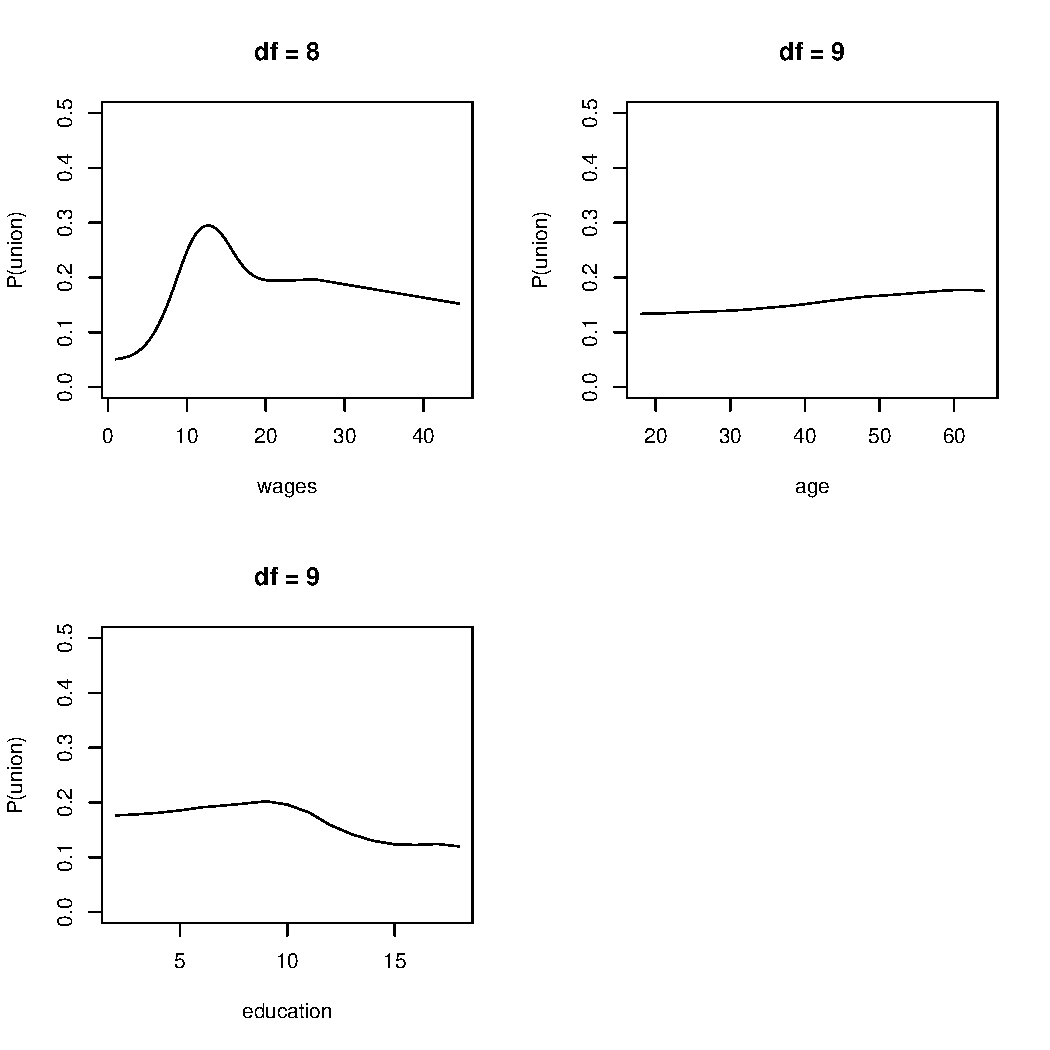
\includegraphics[width=6in]{union_fig.pdf}
\caption{Probablity of membership as a function of covariates. In each plot,
the remaining covariates are fixed at their sample means. The effective
degrees of freedom (df) are also given \protect\cite{hast:tibs:1990}.}
\label{fig:union}
\end{figure}

\subsubsection{The Wage-union data}

The data, which are available from \href{lib.stat.cmu.edu/}{Statlib}, contain
information for each of 534 workers about whether they are members ($y_{i}=1$)
of a workers union or are not ($y_{i}=0$). We study the probability of
membership as a function of six covariates. Expressed in the notation used by
the R (S-Plus) function \texttt{gam}, the model is:
\begin{verbatim}
  union ~race + sex + south + s(wage) + s(age) + s(ed), family=binomial
\end{verbatim}

Here, \texttt{s()} denotes a spline functions with 20 knots each. For
\texttt{wage}, a cubic spline is used, while for \texttt{age} and \texttt{ed},
quadratic splines are used. The total number of random effects that arise from
the three corresponding $\mathbf{u}$ vectors is~64. Figure~\ref{fig:union} shows
the estimated nonparametric components of the model. The time taken to fit the
model was 165~seconds.

\subsubsection{Extensions}

\begin{itemize}
  \item The linear predictor may be a mix of ordinary regression terms
  ($f_{j}(x)=\beta _{j}x$) and nonparametric terms. \scAR\ offers a unified
  approach to fitting such models, in which the smoothing parameters $\lambda
  _{j}$ and the regression parameters $\beta _{j}$ are estimated simultaneously.

  \item It is straightforward in \scAR\ to add ``ordinary'' random effects to
  the model, for instance, to accommodate for correlation within groups of
  observations, as in \citeasnoun{lin:zhan:1999}.
\end{itemize}

See the files
\href{http://otter-rsch.com/admbre/examples/union/union.html}{here}.

\subsection{Semi-parametric estimation of mean and variance}
\label{sec:lidar}
\index{nonparametric estimation!variance function}

\subsubsection{Model description}
An assumption underlying the ordinary regression
\[
y_{i}=a+bx_{i}+\varepsilon _{i}^{\prime }
\]
is that all observations have the same variance, i.e.,
Var$\left( \varepsilon_{i}^{\prime }\right) =\sigma^{2}$. This assumption does
not always hold, e.g., for the data shown in the upper panel of
Figure~\ref{fig:lidar}. This example is taken
from~\citeasnoun{rupp:wand:carr:2003}.

It is clear that the variance increases to the right (for large values of~$x$).
It is also clear that the mean of~$y$ is not a linear function of~$x$. We thus
fit the model
\[
y_{i}=f(x_{i})+\sigma (x_{i})\varepsilon _{i},
\]
where $\varepsilon _{i}\sim N(0,1),$ and $f(x)$ and $\sigma (x)$ are modelled
nonparametrically. We take~$f$ to be a penalized spline. To ensure that $\sigma
(x)>0$, we model $\log \left[ \sigma (x)\right] $, rather than $\sigma (x)$, as
a spline function. For~$f$, we use a cubic spline (20 knots) with a second-order
difference penalty%
\[
-\lambda ^{2}\sum_{k=3}^{20}\left( u_{j}-2u_{j-1}+u_{j-2}\right) ^{2},
\]
while we take $\log \left[ \sigma (x)\right]$ to be a linear spline (20 knots)
with the first-order difference penalty (see equation~(\ref{eqn:first_order})).

\subsubsection{Implementation details}

Details on how to implement spline components are given in Example
\ref{sec:gam}.

\begin{itemize}
  \item Parameters associated with $f$ should be given ``phase~1'' in \scAB,
  while those associated with~$\sigma $ should be given ``phase~2.'' The reason
  is that in order to estimate the variation, one first needs to have fitted the
  mean part.

  \item In order to estimate the variation function, one first needs to have
  fitted the mean part. Parameters associated with~$f$ should thus be given
  ``phase 1'' in \scAB, while those associated with $\sigma$ should be given
  ``phase 2.''
\end{itemize}

\begin{figure}[h]
  \centering\hskip1pt
  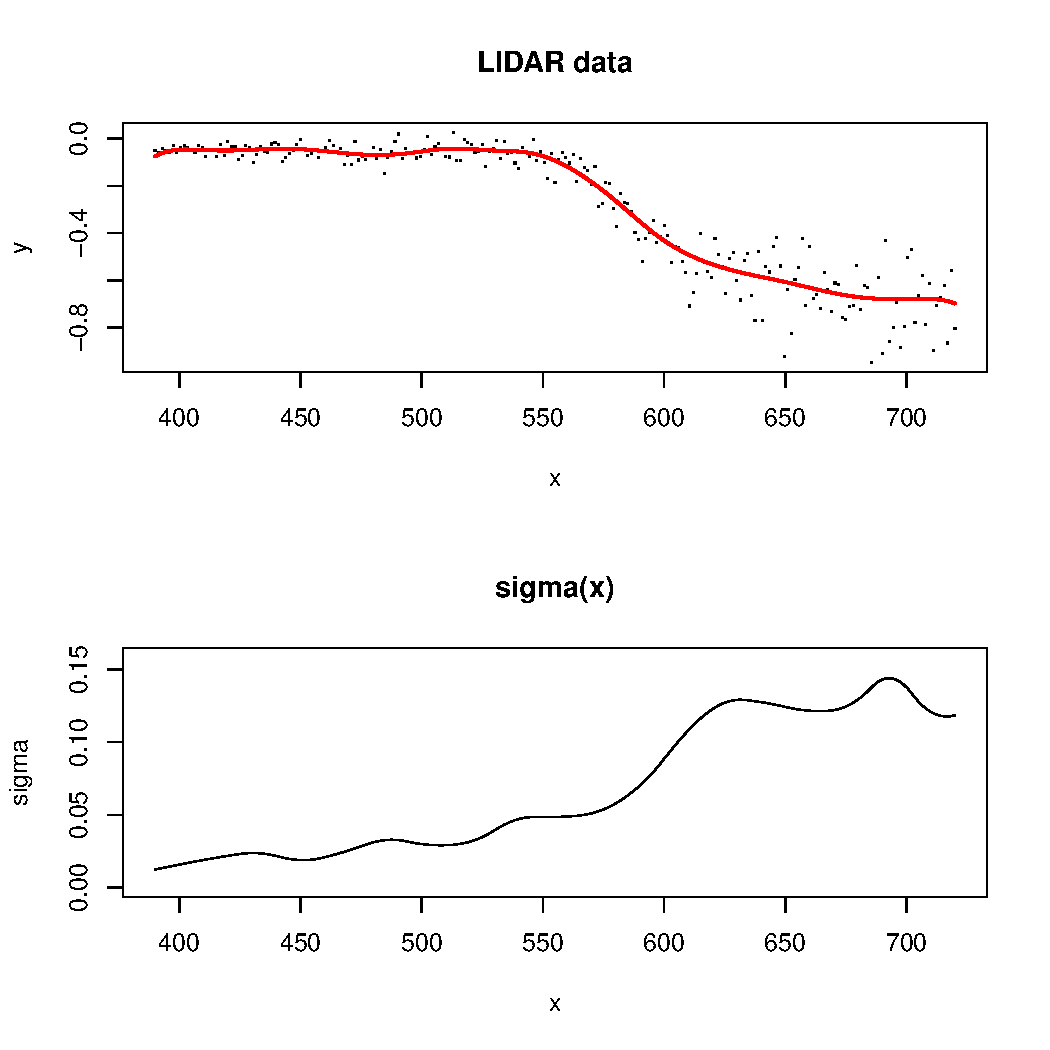
\includegraphics[width=4in]{lidar_fig.pdf}
   \caption{\scLIDAR\ data (upper panel) used by
     \protect\citeasnoun{rupp:wand:carr:2003}, with fitted mean. Fitted standard
     deviation is shown in the lower panel.}
  \label{fig:lidar}
\end{figure}

See the files
\href{http://otter-rsch.com/admbre/examples/lidar/lidar.html}{here}.

\subsection{Weibull regression in survival analysis}
\subsubsection{Model description}

\label{sec:kidney_example}
A typical setting in survival analysis is that we observe the time point~$t$ at
which the death of a patient occurs. Patients may leave the study (for some
reason) before they die. In this case, the survival time is said to be
``censored,'' and~$t$ refers to the time point when the patient left the study.
The indicator variable~$\delta$ is used to indicate whether~$t$ refers to the
death of the patient ($\delta=1$) or to a censoring event ($\delta=0$). The key
quantity in modelling the probability distribution of~$t$ is the hazard
function~$h(t)$, which measures the instantaneous death rate at time~$t$. We
also define the cumulative hazard function $\Lambda(t)=\int_0^t \,
h(s)\,\textrm{ds}$, implicitly assuming that the study started at time $t=0$.
The log-likelihood contribution from our patient is $\delta\log(h(t))-H(t)$. A
commonly used model for $h(t)$ is Cox's proportional hazard model, in which the
hazard rate for the $i^{\textrm{th}}$ patient is assumed to be on the form
\[
  h_it = h_0(t)\exp(\eta_i\mathbf), \qquad i=1,\ldots n.
\]
Here, $h_0(t)$ is the ``baseline'' hazard function (common to all patients) and
$\eta_i=\mathbf{X}_i\mathbf{\beta}$, where $\mathbf{X}_i$ is a covariate vector
specific to the $i^{\textrm{th}}$ patient and $\mathbf{\beta}$ is a vector of
regression parameters. In this example, we shall assume that the baseline hazard
belongs to the Weibull family: $h_0(t)=rt^{r-1}$ for~$r>0$.

In the collection of examples following the distribution of \scWinBUGS, this
model is used to analyse a data set on times to kidney infection for a set of
$n=38$ patients (see \textit{Kidney:\ Weibull regression with random effects} in
the Examples list at
\href{http://www.mrc-bsu.cam.ac.uk/bugs/examples/readme.shtml}%
{The Bugs Project}). The data set contains two observations per patient (the
time to first and second recurrence of infection). In addition, there are three
covariates: \emph{age} (continuous), \emph{sex} (dichotomous), and
\emph{type of disease} (categorical, four levels). There is also an
individual-specific random effect $u_i\sim N(0,\sigma^2)$. Thus, the linear
predictor becomes
\[
  \eta_i = \beta_0 + \beta_\mathrm{sex} \cdot  \mathrm{sex}_i +
  \beta_\mathrm{age} \cdot \mathrm{age}_i +
  \mathbf{\beta}_\mathrm{D}\,\mathbf{x}_i + u_i,
\]
where $\mathbf{\beta}_\mathrm{D}=(\beta_1,\beta_2,\beta_3)$ and $\mathbf{x}_i$
is a dummy vector coding for the disease type. Parameter estimates are shown in
Table~\ref{kidney-parameter-estimates}.
\begin{table}[h]
\begin{center}
  %\footnotesize
  \begin{tabular}{@{\vrule height 12pt depth 6pt width0pt} lrrrrrrrr}
    \hline
               & $\beta_0$ & $\beta_\mathrm{age}$ & $\beta_1$ & $\beta_2$
               & $ \beta_3$ & $\beta_\mathrm{sex}$ & $r$    & $\sigma$\\
    \hline\\[-16pt]
    \scAR\     & -4.3440   & 0.0030               & 0.1208    & 0.6058
    & -1.1423    & -1.8767              & 1.1624 & 0.5617  \\
    Std.\ dev. &  0.8720   & 0.0137               & 0.5008    & 0.5011
    &  0.7729    &  0.4754              & 0.1626 & 0.2970  \\
    BUGS       & -4.6000   & 0.0030               & 0.1329    & 0.6444
    & -1.1680    & -1.9380              & 1.2150 & 0.6374  \\
    Std.\ dev. &  0.8962   & 0.0148               & 0.5393    & 0.5301
    &  0.8335    &  0.4854              & 0.1623 & 0.3570  \\
    \hline
  \end{tabular}
\end{center}
\caption{Parameter estimates for Weibull regression with random effects.}
\label{kidney-parameter-estimates}
\end{table}
See the files
\href{http://otter-rsch.com/admbre/examples/kidney/kidney.html}{here}.

\section{Block-diagonal Hessian}

This section contains models with grouped or nested random effects.

\subsection{Nonlinear mixed models: an \scNLME\ comparison}
\label{sec:orange}

\subsubsection{Model description}

The orange tree growth data was used by \citeasnoun[Ch.8.2]{pinh:bate:2000} to
illustrate how a logistic growth curve model with random effects can be fit with
the S-Plus function \texttt{nlme}. The data contain measurements made at seven
occasions for each of five orange trees. See Table~\ref{tab:orange-trees}.
\begin{table}[h]
\begin{center}
\begin{tabular}{ll}
$t_{ij}$
& Time point when the $j^{\textrm{th}}$ measurement was made on tree~$i$. \\
$y_{ij}$
& Trunk circumference of tree $i$ when measured at time point~$t_{ij}$.
\end{tabular}
\end{center}
\caption{Orange tree data.}
\label{tab:orange-trees}
\end{table}
The following logistic model is used:
\[
y_{ij}=\frac{\phi_{1}+u_i}{1+\exp \left[ -\left( t_{ij}-\phi_{2}\right)
/\phi_{3}\right] }+\varepsilon_{ij},
\]%
where $(\phi_{1},\phi_{2},\phi_{3})$ are hyper-parameters, and
$u_i\sim N(0,\sigma_{u}^{2})$ is a random effect, and
$\varepsilon_{ij}\sim N(0,\sigma ^{2})$ is the residual noise term.

\subsubsection{Results}

Parameter estimates are shown in Table~\ref{tab:parameter-estimates}.
\begin{table}[h]
  \begin{center}
  \begin{tabular}{@{\vrule height 12pt depth 6pt width0pt} llllll}
   \hline
& $\phi_{1}$ & $\phi_{2}$ & $\phi_{3}$ & $\sigma $ & $\sigma_{u}$ \\
  \hline\\[-16pt]
  \scAR\ & 192.1 & 727.9 & 348.1 & 7.843 & 31.65 \\
  Std. dev. & 15.658 & 35.249 & 27.08 & 1.013 & 10.26 \\
  \texttt{nlme} & 191.0 & 722.6 & 344.2 & 7.846 & 31.48 \\
   \hline
  \end{tabular}
  \end{center}
  \caption{Parameter estimates.}
  \label{tab:parameter-estimates}
\end{table}
The difference between the estimates obtained with \scAR\ and \texttt{nlme} is
small. The difference is caused by the fact that the two approaches use
different approximations to the likelihood function. (\scAR\ uses the Laplace
approximation, and for \texttt{nlme}, the reader is referred to~\cite[Ch.
7]{pinh:bate:2000}.)

The computation time for \scAB\ was 0.58~seconds, while the computation time for
\texttt{nlme} (running under S-Plus~6.1) was 1.6~seconds.

See the files
\href{http://otter-rsch.com/admbre/examples/orange/orange.html}{here}.

\subsection{Pharmacokinetics: an \scNLME\ comparison}
\label{sec:pheno}

\subsubsection{Model description}

The ``one-compartment open model'' is commonly used in pharmacokinetics. It can
be described as follows. A patient receives a dose~$D$ of some substance at
time~$t_{d}$. The concentration~$c_t$ at a later time point~$t$ is governed by
the equation
\[
c_t=\tfrac{D}{V}\exp \left[ -\tfrac{Cl}{V}(t-t_{d})\right]
\]
where $V$ and $Cl$ are parameters (the so-called ``Volume of concentration'' and
the ``Clearance''). Doses given at different time points contribute additively
to~$c_t$. \citeasnoun[Ch.~6.4]{pinh:bate:2000} fitted this model to a data set
using the S-Plus routine \texttt{nlme}. The linear predictor used by
\citeasnoun[p.~300]{pinh:bate:2000} is:
\begin{align*}
\log \left( V\right) &=\beta_{1}+\beta_{2}Wt+u_{V}, \\
\log \left( Cl\right) &=\beta_{3}+\beta_{4}Wt+u_{Cl},
\end{align*}
where $Wt$ is a continuous covariate, while $u_{V}\sim N(0,\sigma_{V}^{2})$ and
$u_{Cl}\sim N(0,\sigma_{Cl}^{2})$ are random effects. The model specification is
completed by the requirement that the observed concentration~$y$ in the patient
is related to the true concentration by $y=c_t+\varepsilon $, where $\varepsilon
\sim N(0,\sigma ^{2})$ is a measurement error term.

\subsubsection{Results}

Estimates of hyper-parameters are shown in Table~\ref{tab:hyper-estimates}.
\begin{table}[h]
\begin{center}
\begin{tabular}{@{\vrule height 12pt depth 6pt width0pt} llllllll}
 \hline
& $\beta_{1}$ & $\beta_{2}$ & $\beta_{3}$ & $\beta_{4}$ & $\sigma $ & $
\sigma_{V}$ & $\sigma_{Cl}$ \\
 \hline\\[-17pt]
\scAR\ & -5.99 & 0.622 & -0.471 & 0.532 & 2.72 & 0.171 & 0.227 \\
Std. Dev & 0.13 & 0.076 & 0.067 & 0.040 & 0.23 & 0.024 & 0.054 \\
\texttt{nlme} & -5.96 & 0.620 & -0.485 & 0.532 & 2.73 & 0.173 & 0.216\\
 \hline
\end{tabular}
\end{center}
\caption{Hyper-parameter estimates: pharmacokinetics.}
\label{tab:hyper-estimates}
\end{table}
The differences between the estimates obtained with \scAR\ and \texttt{nlme} are
caused by the fact that the two methods use different approximations of the
likelihood function. \scAR\ uses the Laplace approximation, while the method
used by \texttt{nlme} is described in~\citeasnoun[Ch.~7]{pinh:bate:2000}.

The time taken to fit the model by \scAR\ was 17~seconds, while the computation
time for \texttt{nlme} (under S-Plus~6.1) was 7~seconds.

See the files
\href{http://otter-rsch.com/admbre/examples/pheno/pheno.html}{here}.

\subsection{Frequency weighting in \scAR}
\label{seq:frequency_example}

\subsubsection{Model description}

Let $X_{i}$ be binomially distributed with paramters $N=2$ and $p_{i}$, and
further assume that
\begin{equation}
p_{i}=\frac{\exp (\mu +u_{i})}{1+\exp (\mu +u_{i})},
\end{equation}%
where $\mu $ is a parameter and $u_{i}\sim N(0,\sigma ^{2})$ is a random effect.
Assuming independence, the log-likelihood function for the parameter $\theta
=(\mu ,\sigma )$ can be written as
\begin{equation}
l(\theta )=\sum_{i=1}^{n}\log \bigl[\, p(x_{i};\theta )\bigr] .
\end{equation}%
In \scAR, $p(x_{i};\theta )$ is approximated using the Laplace approximation.
However, since $x_{i}$ only can take the values~$0$, $1$, and~$2$, we can
rewrite the log-likelihood as
\begin{equation}
l(\theta )=\sum_{j=0}^{2}n_{j}\log \bigl[\, p(j;\theta )\bigr] ,  \label{l_w}
\end{equation}%
where $n_{j}$ is the number $x_{i}$ being equal to~$j$. Still, the Laplace
approximation must be used to approximate $p(j;\theta )$, but now only for
$j=0,1,2$, as opposed to $j = 1,\dots n$, as above. For large~$n$, this can give
large savings.

To implement the log-likelihood (\ref{l_w}) in \scAR, you must organize your
code into a \texttt{SEPARABLE\_FUNCTION} (see the section ''Nested models'' in
the \scAR\ manual). Then you should do the following:
\begin{itemize}
\item Formulate the objective function in the weighted form (\ref{l_w}).

\item Include the statement
  \begin{lstlisting}
  !! set_multinomial_weights(w);
  \end{lstlisting}
in the \texttt{PARAMETER\_SECTION}. The variable \texttt{w} is a vector (with
indexes starting at~1) containing the weights, so in our case,
$w=(n_{0},n_{1},n_{2})$.
\end{itemize}

See the files
\href{http://otter-rsch.com/admbre/examples/weights/weights.html}{here}.

\subsection{Ordinal-logistic regression}
\label{sec:socatt_example}

\subsubsection{Model description}

In this model, the response variable $y$ takes on values from the ordered set
$\{y^{(s)},s=1,\ldots,S-1\}$, where $y^{(1)}<y^{(2)}<\cdots<y^{(S)}$. For
$s=1,\ldots,S-1$, define $P_s=P(y\leq y^{(s)})$ and $\kappa_s=\log
[P_s/(1-P_s)]$. To allow $\kappa_s$ to depend on covariates specific to the
$i^{\textrm{th}}$ observation ($i=1,\ldots,n$), we introduce a
disturbance~$\eta_i$ of~$\kappa_s$:
\[
  P(y_i\leq y^{(s)}) =
  \frac{\exp(\kappa_s-\eta_i)}
  {1+\exp(\kappa _{s}-\eta _{i})}, \qquad s=1,\ldots,S-1.
\]
with
\[
  \eta_i = \mathbf{X}_i\mathbf{\beta}+u_{j_i},
\]
where $\mathbf{X}_i$ and $\mathbf{\beta}$ play the sample role, as in earlier
examples. %Example~1-3
The $u_j$ ($j=1,\ldots,q$) are independent $N(0,\sigma^2)$ variables, and $j_i$
is the latent variable class of individual~$i$.

See the files
\href{http://otter-rsch.com/admbre/examples/socatt/socatt.html}{here}.

\section{Banded Hessian (state-space)}

Here are some examples of state-space models.

\subsection{Stochastic volatility models in finance}

\subsubsection{Model description}

Stochastic volatility models are used in mathematical finance to describe the
evolution of asset returns, which typically exhibit changing variances over
time. As an illustration, we use a time series of daily pound/dollar exchange
rates~$\{z_t\}$ from the period 01/10/81 to 28/6/85, previously analyzed
by~\citeasnoun{harv:ruiz:shep:1994}. The series of interest are the daily
mean-corrected returns~$\{y_t\}$, given by the transformation
\[
  y_t = \log z_t - \log z_{t-1} - n^{-1}\sum_{i=1}^n(\log z_t-\log z_{t-1}).
\]

The stochastic volatility model allows the variance of~$y_t$ to vary smoothly
with time. This is achieved by assuming that $yt\sim N(\mu,\sigma_t^2)$, where
$\sigma_t^2=\exp(\mu_x+x_t)$. The smoothly varying component~$x_t$ follows the
autoregression
\[
  x_t = \beta x_{t-1} + \varepsilon_t, \qquad \varepsilon_t \sim N(0,\sigma^2).
\]

The vector of hyper-parameters is for this model is thus
$(\beta,\sigma,\mu,\mu_x)$.

See the files \href{http://otter-rsch.com/admbre/examples/sdv/sdv.html}{here}.

\subsection{A discrete valued time series: the polio data set}
\label{sec:sdv_example}

\subsubsection{Model description}

\citeasnoun{zege:1988} analyzed a time series of monthly numbers of
poliomyelitis cases during the period 1970--1983 in the U.S. We make a
comparison to the performance of the Monte Carlo Newton-Raphson method, as
reported in~\citeasnoun{kuk:chen:1999}. We adopt their model formulation.

Let $y_{i}$ denote the number of polio cases in the $i^{\textrm{th}}$ period
$(i=1,\ldots,168)$. It is assumed that the distribution of~$y_{i}$ is governed
by a latent stationary AR(1) process~$\{u_i\}$ satisfying
\[
  u_i = \rho u_{i-1} + \varepsilon_i,
\]
where the $\varepsilon_i\sim N(0,\sigma^2)$. % variables.
To account for trend and seasonality, the following covariate vector is
introduced:
\[
  \mathbf{x}_i = \Bigg(
    1,
    \frac{i}{1000},
    \cos\left(\frac{2\pi}{12}i\right),
    \sin\left(\frac{2\pi}{12}i\right),
    \cos\left(\frac{2\pi}{6}i\right),
    \sin\left(\frac{2\pi}{6}i\right)
  \Bigg).
\]

Conditionally on the latent process $\{u_i\}$, the counts $y_i$ are
independently Poisson distributed with intensity
\[
  \lambda_i=\exp(\mathbf{x}_i{}'\mathbf{\beta}+u_i).
\]

\subsubsection{Results}

Estimates of hyper-parameters are shown in Table~\ref{tab:hyper-estimates-2}.
\begin{table}[h]
\begin{center}
  \footnotesize
  \begin{tabular}{@{\vrule height 12pt depth 6pt width0pt} lrrrrrrrr}
    \hline
    ~                          & $\beta_1$ & $\beta_2$ & $\beta_3$ & $\beta_4$
    & $\beta_5$ & $\beta_6$ & $\rho$ & $\sigma$\\
    \hline\\[-16pt]
    \scAR\                     & 0.242     & -3.81     & 0.162     & -0.482
    & 0.413     & -0.0109   & 0.627  & 0.538   \\
    Std.\ dev.                 & 0.270     &  2.76     & 0.150     &  0.160
    & 0.130     &  0.1300   & 0.190  & 0.150   \\
    \citeasnoun{kuk:chen:1999} & 0.244     & -3.82     & 0.162     & -0.478
    & 0.413     & -0.0109   & 0.665  & 0.519   \\
    \hline
  \end{tabular}
\end{center}
\caption{Hyper-parameter estimates: polio data set.}
\label{tab:hyper-estimates-2}
\end{table}

We note that % not
the standard deviation is large for several regression parameters. The \scAR\
estimates (which are based on the Laplace approximation) are very similar to the
exact maximum likelihood estimates, as obtained with the method
of~\citeasnoun{kuk:chen:1999}.

See the files
\href{http://otter-rsch.com/admbre/examples/polio/polio.html}{here}.

\section{Generally sparse Hessian}

\subsection{Multilevel Rasch model}

The multilevel Rasch model can be implented using random effects in \scAB. As an
example, we use data on the responses of 2042~soldiers to a total of 19~items
(questions), taken from~\cite{doran2007estimating} %Doran et al.\ (2007).
This illustrates the use of crossed random effects in \scAB. Furthermore, it is
shown how the model easily can be generalized in \scAB. These more general
models cannot be fitted with standard \scGLMM\ software, such as ``lmer'' in~R.

See the files \href{http://admb-project.org/community/tutorials-and-examples/%
random-effects-example-collection/%
item-response-theory-irt-and-the-multilevel-rasch-model-1}{here}.

\chapter{Differences between \scAB\ and \scAR?}

\begin{itemize}
\item Profile likelihoods are now implemented also in random effects models, but with
     the limitation that the \texttt{likeprof\_number} can only depend on parameters,
     not random effects. 
\item Certain functions, especially for matrix operations, have not been
implemented.
\item The assignment operator for \texttt{dvariable} behaves differently. The
code
\begin{lstlisting}
     dvariable y = 1;
     dvariable x = y;
\end{lstlisting}
will make \texttt{x} and \texttt{y} point to the same memory location (shallow
copy) in \scAR. Hence, changing the value of \texttt{x} automatically changes
\texttt{y}. Under \scAB, on the other hand, \texttt{x} and \texttt{y} will refer
to different memory locations (deep copy). If you want to perform a deep copy
in \scAR\ you should write:
\begin{lstlisting}
     dvariable y = 1;
     dvariable x;
     x = y;
\end{lstlisting}
For vector and matrix objects \scAB\ and \scAR\ behave identically in that
a shallow copy is used.
\end{itemize}

\chapter{Command Line options}
\label{sec:command_line_options}
\index{command line options!\scAR-specific}

A list of command line options accepted by \scAB\ programs can be obtained using
the command line option \texttt{-?}, for instance,
\begin{lstlisting}
  $ simple -?
\end{lstlisting}
Those options that are specific to \scAR\ are printed after line the ``Random
effects options if applicable.'' See Table~\ref{tab:command-line-options}.
\begin{table}[h]
\begin{center}
\begin{tabular*}{.95\textwidth}%
{@{\vrule height 14pt depth 10pt width0pt}@{\extracolsep{1em}} l
  p{.8\textwidth} }
\hline
\textbf{Option}& \textbf{Explanation}\\[-3pt]
\hline
\hline
\texttt{-nr N}     & maximum number of Newton-Raphson steps\\
\texttt{-imaxfn N}
& maximum number of evals in quasi-Newton inner optimization\\
\texttt{-is N}
& set importance sampling size to \texttt{N} for random effects\\
\texttt{-isf N}
& set importance sampling size funnel blocks to \texttt{N} for random effects\\
\texttt{-isdiag}   & print importance sampling diagnostics\\
\texttt{-hybrid}   & do hybrid Monte Carlo version of \scMCMC\\
\texttt{-hbf}      & set the hybrid bounded flag for bounded parameters\\
\texttt{-hyeps}    & mean step size for hybrid Monte Carlo\\
\texttt{-hynstep}  & number of steps for hybrid Monte Carlo\\
\texttt{-noinit}   & do not initialize random effects before inner optimzation\\
\texttt{-ndi N}    & set maximum number of separable calls\\
\texttt{-ndb N}
& set number of blocks for derivatives for random effects (reduces temporary
file sizes)\\
\texttt{-ddnr}
& use high-precision Newton-Raphson for inner optimization for banded
\mbox{Hessian} case \textit{only}, even if implemented\\
\texttt{-nrdbg}    & verbose reporting for debugging Newton-Raphson\\
\texttt{-mm N}     & do minimax optimization\\
\texttt{-shess}    & use sparse Hessian structure inner optimzation\\
\hline
\texttt{-l1 N}  & set the size of buffer \texttt{f1b2list1} to~\texttt{N}  \\
\texttt{-l2 N}  & set the size of buffer \texttt{f1b2list12} to~\texttt{N} \\
\texttt{-l3 N}  & set the size of buffer \texttt{f1b2list13} to~\texttt{N} \\
\texttt{-nl1 N} & set the size of buffer \texttt{nf1b2list1} to~\texttt{N} \\
\texttt{-nl2 N} & set the size of buffer \texttt{nf1b2list12} to~\texttt{N}\\
\texttt{-nl3 N}
& set the size of buffer \texttt{nf1b2list13} to~\texttt{N} \\\hline
\end{tabular*}
\end{center}
\caption{Command line options.}
\label{tab:command-line-options}
\end{table}
The options in the last section (the sections are separated by horizontal bars)
are not printed, but can still be used (see earlier).

\chapter{Quick References}\label{ch:05}
\label{sec:quick}

\section{Compiling \scAB\ programs}
\label{sec:compiling}

To compile \texttt{model.tpl} in a \textsc{DOS}/Linux terminal window, type
\begin{code}
  admb [-s] [-re] model
\end{code}
where the options
\par
\begin{tabular}{@{\texttt} l l }
  -s & yields the ``safe'' version of the \textsc{exe} file\\
  -re & is used to invoke the random effect module
\end{tabular}

\medskip

\noindent There are two stages of compilation:
\begin{itemize}
  \item Proprocessor: \texttt{tpl2cpp} or \texttt{tpl2rem}
  \item \cplus\ compiler (Borland, Visual \cplus, etc.)
\end{itemize}
\begin{center}
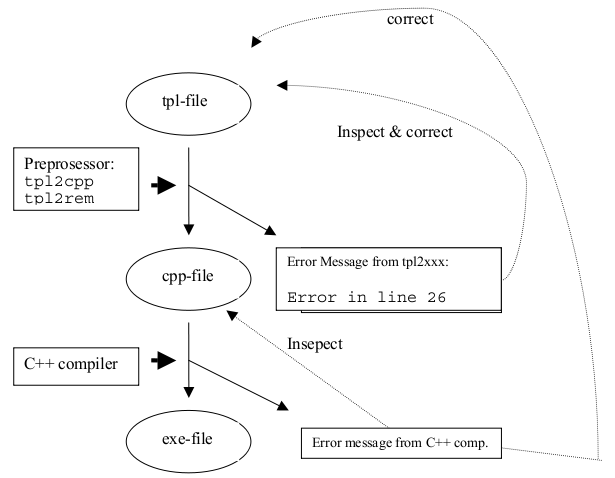
\includegraphics[width=11cm]{compiling-diagram.png}
\end{center}

\hskip-2pc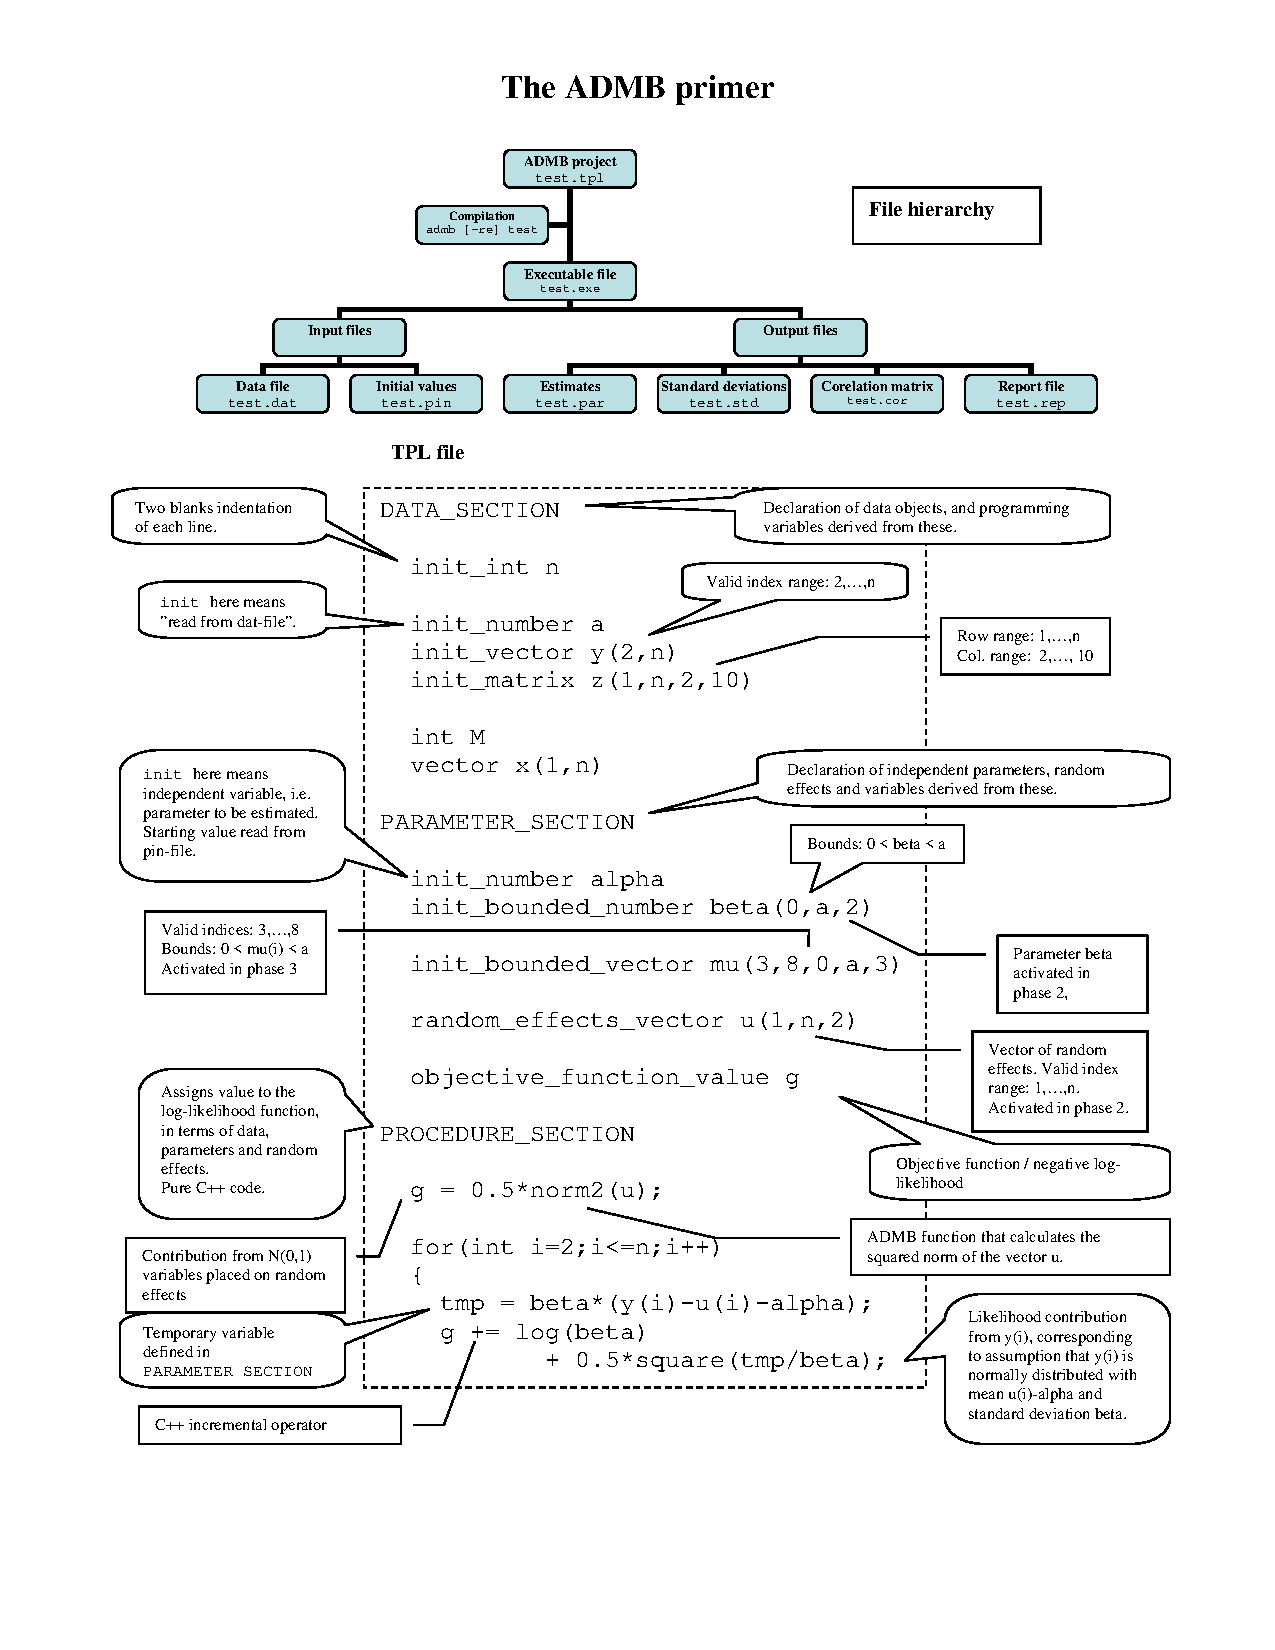
\includegraphics[width=18cm]{ADMBprim.pdf}%17

\bibliographystyle{plain}
\bibliography{admbre}

\printindex

\end{document}
